\chapter{Methods}

%TODO: IST KLAR GENUG: "ich replizier diese 3 algorithmen, aus diesen 3 papern"

This chapter explains the methods that were used to achieve the two goals of replicating the algorihm of \textcite{Derrac2015} with the improvements of \cite{Ager2018,Alshaikh2020} with a sustainable architecture and applying it to the domain of educational resources.  

To do that, we will firstly look at the datasets \mainalgos used as well as our own dataset and compare key statistics. The subsequent section then explains the used algorithm broadly before looking at each of its steps in detail. Based on that, the specific architecture that was created as well as the workflow used to generate meaningful results will be introduced to demonstrate its process. The final section explains what kind of methods and metrics were used to generate and interpret the results that will follow in the next chapter.

Given that there were two research questions, one asking if the replicating algorithm can be applied to another domain and the other asking for a reliable application, it makes sense to both look at datasets and general algorithm on the one side, but also at the worflow and architecture. Writing about the latter while also open-sourcing the code-base is especially useful to ensure ease and speed of future replication, such that all claims can be independently tested with the exact same implementation without having to rely on ambiguous and incomplete verbal explanations\footnote{Just like this thesis could have been a lot less effort if \mainalgos did that instead of ambiguous incomplete descriptions. \todoparagraph{Scable, reproducible, open science! I wished it had been there, so I will do it.}}. 


%JOHANNES' KOMMENTARE TO WHAT I SENT HIM
% * Starker Unterschied zwischen Theoretisch (Dataset,..) und implementation unten in Terms of Verständlichkeit.
% => Implementation extrem verständlich, erster teil (dataset+algo) "teilweise unverstädnlich"
% * Struktur mit den Subsections so sinnvoll. Aber Streamlinen:
% * Verhältnis von Datensatz und Algo wird nicht klar und von den einzelnnen Datensätzen (am anfang sag ich ja es gibt das eine mit den 15.000 und beim zweiten sag ich goar nix dazu)


\section{Datasets}


%TODO: wird klar genug "Die 3 haupt-autoren nutzen halt diesen algo auf diesen datasets, ich will domänentransfer machen, daher macht es sinn zu gucken ob die grundlegend unterschiedlich sind"
% -> damit auch main-claim (Kommentar Johannes, es war sehr unklar welche datasets mich inwieweit interessieren und warum ich die beschreib die ich beschreib)
% * Verhältnis von Datensatz und Algorithmus wird nicht klar
% * Warum ich die einzelnen Datensätze erwähne wird nicht klar


Let us first elaborate on the datasets used both in the works that are being replicated as well as the dataset used in the scope of this thesis. Doing both is important because (as explained in \autoref{sec:howtoreplicate}), to really know if an algorithm is a good choice for a task, it must be ensured that it does not only work on a special kind of dataset due to a special property that this kind of data happens to have. So, we will now compare all datasets, to see if there are important differences between them, as for example in its structure, size or just general \emph{logic}.

\textcite{Derrac2015} used their algorithm to create conceptual spaces for three domains: \textit{movies}, \textit{placetypes} and \textit{wines}. Accordingly, they created corpora for these three domains. The two considered follow-up works both re-used the datasets for movies and placetypes and also created additional datasets respectively. An overview of all the corpora used in \mainalgos is provided in \autoref{tab:all_datasets}.

% NOW at first the ones from \mainalgos I am using

\subsection*{Comparing dataset properties}

This work applies the replicated algorithm to a new dataset, so it is important to check if the new dataset differs from the originally used ones. To ensure comparability in algorithm details, this implementation is also run on the \emph{placetypes}-dataset, and some of its statistics as well as that of the other two datasets made public by \cite{Derrac2015}\footnote{\url{https://www.cs.cf.ac.uk/semanticspaces/}}. Let us first compare some key statistics of them, before looking into two of them individually in the next section.

A very distinctive difference of the datasets is their size: the movies-dataset consists of 15.000 entities, place-types of 1383, and wines of only 330. Just as important as the number of entities is however also the length of their associated text-corpus. Figures \ref{fig:sid_wordsperdesc} and \ref{fig:placetypes_dist_unique} show a histogram of the distribution of text lengths for the Siddata-dataset and placetypes-dataset respectively, and \autoref{tab:corpussizes} summarize corpus size and distribution of text lengths per entity for all handled datasets. Note that the Siddata-dataset is listed twice, once including all available entities and once after filtering out those whose description was shorter than 80 words.

\begin{table}[H]
	\centering
	\begin{tabular}{r|l|lll|lll}
		&  \textbf{Entities}   & \multicolumn{6}{c}{\textbf{Words per Entity}}                                 \\
		&       & \multicolumn{3}{c}{\textbf{Unique}} & \multicolumn{3}{c}{\textbf{Non-Unique}} \\
	 &  & \textbf{5\textsuperscript{th}} & \textbf{Med} & \textbf{95\textsuperscript{th}} & \textbf{5\textsuperscript{th}} & \textbf{Med} & \textbf{95\textsuperscript{th}} \\ \midrule
	\textbf{movie reviews}                                                          & 13978 & 565       & 1358       & 5510       & 962        & 3179        & 38378        \\
	\textbf{place types}                                                          & 1383  & 159       & 2215       & 18117      & 2378       & 55422       & 886233       \\
	\textbf{Siddata (all)}     & 26346 & 19        & 60         & 169        & 22         & 71          & 239          \\
	\textbf{Siddata} ($\geq 80$ words) & 11601 & 63        & 99         & 211        & 83         & 124         & 323         
	\end{tabular}
	\caption{Sizes of the text-corpora of the Siddata-dataset and those of \cite{Derrac2015}. The columns \textit{Words per Entity} list the 5\textsuperscript{th}, 50\textsuperscript{th}, and 95\textsuperscript{th} percentile respectively.}
	\label{tab:corpussizes}
\end{table}

It is obvious that even though the number of Siddata-entities is comparable to the bigger of \cite{Derrac2015}'s datasets, the number of unique words in the individual texts associated with the entities are two orders of magnitude shorter than both. As the algorithm does not rely on deep learning, this does not mean that the dataset is unsuited for it, but let us explore how the distance in their lengths can be explained and what consequences this has.

The works considered in this replication \mainalgos all use the movies- and the  placetypes-dataset to evaluate their methods. The former consists of the concatenation of all available reviews for 15.000 movies from IMDB\footnote{\url{https://www.imdb.com/}}, grouped by the movie the reviews are for. The placetypes-dataset is created from a collection of tags that belong to photos uploaded to the photo sharing platform Flickr\footnote{\url{https://www.flickr.com}} that co-occur with other tags that denote one of several placetypes. Other datasets considered in the works of \mainalgos include wine reviews, posts to certain newsgroups, and another dataset created from IMDB-reviews (see \tref{tab:all_datasets}). 
% "their algorithm is tailored to concatenated-reviews or concatenated-bags-of-tags"

All of these datasets have in common that they are made up from a collection of independent texts or tags, created by different people. This means, that the more obvious or distinct a property of the respective entity is, the more often words describing that property will be used as tag or as part of the review. For example, a movie that is \emph{scary} to a lot of people will lead to many reviews mentioning that, which means that the word scary (or other words commonly co-occuring with it) will have a high count in the concatenation of all these reviews. The algorithm from \cite{Derrac2015} heavily leans on this property by using the (relative) frequency of certain words as signal for the importance of the concept they may refer to. 

The Siddata-dataset unfortunately does not share this property, as the texts that belong to an entity are not collected from different independent texts, but solely from the description of that entity. It may of course be roughly the case that the more \emph{mathematical} a course is, the more often the word \emph{math} occurs in its description, but the correlation is likely not as prominent as in the aforementioned datasets. It should however be noted that \cite{Alshaikh2020} also used the algorithm on three datasets where the description for an entity was collected from its Wikipedia\footnote{\url{https://en.wikipedia.org/}}-article, which also does not contain the described duplication of words. \autoref{tab:all_datasets} shows a complete comparison of all datasets used in any of \mainalgos, including their origin, properties as well as associated pre-processing steps.

%TODO https://tex.stackexchange.com/questions/526198/table-resize-table-and-automatic-line-breaks
%TODO add back key feature sizes?!

% \afterpage{%

\newgeometry{
	a4paper,
	top=18mm,
	bottom=8mm,
} 
\clearpage

\begin{landscape}
	\begin{table}[]
		\resizebox{\textwidth}{!}{%
			\begin{tabular}{@{}lllllll@{}} 
				\toprule
					\textbf{dataset} &
					\textbf{contents} &
					\textbf{preprocessing} &
					\textbf{size} &
					\textbf{classification classes} &
					\textbf{candidate word threshold}
					& \textbf{key feature sizes} 
					 \\ \midrule
				\textbf{movies\footnote{\label{origdsets}\url{https://www.cs.cf.ac.uk/semanticspaces/}} \cite{Derrac2015} \cite{Ager2018} \cite{Alshaikh2020} } &
					grouped-by-movie-concatenated reviews for movies & 
					\specialcell[l]{\tabitem removed stop-words\footnote{\label{fnote:stopwordlist}\url{http://snowball.tartarus.org/algorithms/english/stop.txt}} \\ \tabitem lower-cased text \\ \tabitem removed diacritics  \\ \tabitem removed punctuation} &
					\specialcell[l]{\cite{Derrac2015}: 15000 movies \\ \cite{Ager2018,Alshaikh2020}: 13978 movies } & %Ager2018 says 15.000 - 1022 duplicates, that's the number of Alshaikh2020
					\specialcell[l]{ \tabitem genre (23 classes)\\ \tabitem plot keywords (eg. \textit{suicide, beach}) (100 classes) \\ \tabitem age-rating certificates (6 classes)} & \specialcell[l]{$\geq$ 100 occurences (doq-freq) \\ \textrightarrow around 22k candidates \\ variable-length \textbf{n-grams} considered}
					& \specialcell[l]{feature vecs: 38649 keys with 0-33k terms each (sum: 589727 terms) \\ candidate-terms: 22903 (unclustered)\\ clusters: ndims*2  $\rightarrow$ for 20D: 9389 ($\rightarrow$ 9429 words in $T^{0.1}$)}		
					% movies: 15.000
					% ppmi-weighted feature vectors: 38649 keys with bag-of-words between 0 words and 33k words (but mostly couple 1000s), all in all 589727 unique terms
					% candidate-terms: 22903 (unclustered)
					% clusters: ndims*2 clusters with all in all (for 20d) 9389 values (->9429 words have kappa>=0.5)
					\\ \midrule
				\textbf{place types\footref{origdsets} \cite{Derrac2015} \cite{Ager2018} \cite{Alshaikh2020} } &
					Tags of Flickr-photos that are also tagged with a place-type 
					% bag-of-tags from Flickr used to describe places of a certain place-type
					& 
					None &
					1383 place-types & %both in DESC15 and the follow-up paper
					\specialcell[l]{ \tabitem category from Geonames (7 classes)\\ \tabitem category from Foursquare (9 classes)\\ \tabitem category from OpenCYC (\cite{Derrac2015}: 93 classes, \cite{Ager2018,Alshaikh2020}: 20 classes) } &
					\specialcell[l]{ $\geq$ 50 occurences (doq-freq) \\ \textrightarrow around 22k candidates \\ (all words from the BoW) \\ \textbf{n-grams}: squashed all words of a tag}
					\\ \midrule
				\textbf{wines\footref{origdsets}\footnote{\url{https://snap.stanford.edu/data/web-CellarTracker.html}} \cite{Derrac2015}} &
					grouped-by-wine-variant concatenated reviews for wines & \specialcell[l]{\tabitem removed stop-words\footnoteref{fnote:stopwordlist} \\ \tabitem lower-cased text \\ \tabitem removed diacritics  \\ \tabitem removed punctuation} &
					\textit{not performed} &
					\specialcell[l] {$\geq$ 50 occurences (doq-freq) \\  \textrightarrow around 6k candidates }
					\\ \midrule
				\textbf{20 newsgroups\footnote{\url{http://qwone.com/~jason/20Newsgroups}} \cite{Ager2018}} &
					posts partitioned (nearly) evenly across 20 different newsgroups &
					\specialcell[l]{ \tabitem Headers, footers and quote metadata removed using scikit-learn \footnote{\url{https://scikit-learn.org/0.19/datasets/twenty_newsgroups.html}} \\ \tabitem removed stopwords (using NLTK's corpus \cite{loper-bird-2002-nltk})\\ \tabitem lowercased text\\ \tabitem candidate terms: all textual and numerical tokens} &
					18446 posts &
					\tabitem newgroup post was submitted to (20 classes) &
					$\geq$ 30 occurences 
					\\ \midrule
				\textbf{imdb sentiment\footnote{\url{http://ai.stanford.edu/~amaas/data/sentiment/} \cite{maas-EtAl:2011:ACL-HLT2011}} \cite{Ager2018}} &
					highly polar movie reviews for binary sentiment classification  &
					\specialcell[l]{ \tabitem removed stopwords (using NLTK's corpus \cite{loper-bird-2002-nltk})\\ \tabitem lowercased text\\ \tabitem candidate terms: all textual and numerical tokens} &
					50000 reviews &
					\tabitem sentiment of the review (2 classes) &
					$\geq$ 50 occurences
					\\ \midrule
				\textbf{Bands \cite{Alshaikh2020}} &
					\specialcell[l]{All Wikipedia pages ($\geq$ 200 words) whose \\ WikiData semantic type is "Band"} &
					\specialcell[l]{ \tabitem removed HTML-tags and references \\ \tabitem \textit{"standard preprocessing strategy"} \cite[137]{Alshaikh2019} \\ \tabitem removed stopwords (using NLTK's corpus \cite{loper-bird-2002-nltk})\\ \tabitem POS-tagging and keeping only nouns and adjectives \\ \tabitem remove words with a rel. doc-freq  $>$ 60\% or abs. doc-freq $<$ 10 } &
					11448 bands & \specialcell[l]{ \tabitem Genres (22 classes) \\ \tabitem Country of origin (6 classes) \\ \tabitem Loc. of formation (4 classes) }  & 
					\specialcell[l]{ 10 $<$ doc-freq $<$ 6869 \\ (all words from the BoW)}\\ \midrule
				\textbf{Organisations\footnote{\label{fnote:for_alshaikh2019} Originally created in and for \cite{Alshaikh2019}} \cite{Alshaikh2020}} &
					\specialcell[l]{All Wikipedia pages ($\geq$ 200 words) whose \\ WikiData semantic type is "Organisation"} &
					\specialcell[l]{ \tabitem removed HTML-tags and references \\ \tabitem \textit{"standard preprocessing strategy"} \cite[137]{Alshaikh2019} \\ \tabitem removed stopwords (using NLTK's corpus \cite{loper-bird-2002-nltk})\\ \tabitem POS-tagging and keeping only nouns and adjectives \\ \tabitem remove words with a rel. doc-freq  $>$ 60\% or abs. doc-freq $<$ 10 } &
					11800 organisations &
					\specialcell[l]{ \tabitem Country (4 classes)\\ \tabitem Headquarter Loc. (2 classes)} &
					\specialcell[l]{ 10 $<$ doc-freq $<$ 7080 \\ (all words from the BoW)} \\ \midrule
				\textbf{Buildings\footnoteref{fnote:for_alshaikh2019} \cite{Alshaikh2020}} &
					\specialcell[l]{All Wikipedia pages ($\geq$ 200 words) whose \\ WikiData semantic type is "Building"} &
					\specialcell[l]{ \tabitem removed HTML-tags and references \\ \tabitem \textit{"standard preprocessing strategy"} \cite[137]{Alshaikh2019} \\ \tabitem removed stopwords (using NLTK's corpus \cite{loper-bird-2002-nltk})\\ \tabitem POS-tagging and keeping only nouns and adjectives \\ \tabitem remove words with a rel. doc-freq  $>$ 60\% or abs. doc-freq $<$ 10 } &
					3721 buildings &
					\specialcell[l]{ \tabitem Country (2 classes)\\ \tabitem Administrative loc. (2 classes)} &
					\specialcell[l]{10 $<$ doc-freq $<$ 2233 \\ (all words from the BoW) }\\ \midrule \midrule
				\textbf{Siddata-Courses} &
					TODO &
					&
					&
					\tabitem Faculty (10 classes) 
					\\ \midrule 
				\textbf{100K Coursera reviews}\footnote{\url{https://www.kaggle.com/septa97/100k-courseras-course-reviews-dataset}} &
					TODO &
					&
					&
					\specialcell[l]{ \tabitem Rating (5 classes) \\ \textit{\tabitem Major, Category, Offered-By,... (tbd)} }
					\\ 
			\end{tabular}
			\slcaption{All datasets. Extends similar table in \cite{Alshaikh2020}}
			\label{tab:all_datasets}
		}
	\end{table}
	% TODO was ist mit n>1-grams? Movies used them, placetypes used tags so it kinda has them... and stuff liek buildings/organizations?
\end{landscape}	


\restoregeometry
% } %afterpage

\subsection{SIDDATA-courses}

\label{sec:dataset_siddata}

% Generelle Analyse Datensatz mit Plots (Längenverteilung der Descriptions, ...)
% ich würde SIDDATA immer in caps schreiben wenn du das Projekt meinst, wenn du die software meinst kannst du die ja auch klein introducen bzw die auch mit digital study assistant (DSA) abkürzen

\begin{table}[H]
	\resizebox{\textwidth}{!}{%
	\begin{tabular}{lllllrrrr}
	\toprule
	 &  &  &  &  & \textbf{$\geq$20} & \textbf{$\geq$50} & \textbf{$\geq$200} & \textbf{$\geq$500} \\
	\textbf{Source} & \textbf{Type} & \textbf{Format} & \textbf{Uni} & \textbf{Lang.} &  &  &  &  \\
	\midrule
	\multirow[t]{3}{*}{\textbf{2021 Dump}} & \multirow[t]{3}{*}{\textbf{Stud.IP}} & \multirow[t]{3}{*}{\textbf{Course}} & \multirow[t]{3}{*}{\textbf{\acrshort{uos}}} & \textbf{de} & 18203 & 14551 & 2671 & 100 \\
	 &  &  &  & \textbf{en} & 1950 & 1773 & 616 & 53 \\
	 &  &  &  & \textbf{other} & 681 & 612 & 100 & 1 \\
	\cline{1-5} \cline{2-5} \cline{3-5} \cline{4-5}
	\multirow[t]{6}{*}{\textbf{2022 Dump}} & \multirow[t]{6}{*}{\textbf{Stud.IP}} & \multirow[t]{6}{*}{\textbf{Course}} & \multirow[t]{3}{*}{\textbf{\acrshort{uos}}} & \textbf{de} & 1009 & 807 & 188 & 5 \\
	 &  &  &  & \textbf{en} & 132 & 123 & 70 & 13 \\
	 &  &  &  & \textbf{other} & 20 & 14 & 1 & - \\
	\cline{4-5}
	 &  &  & \multirow[t]{3}{*}{\textbf{other}} & \textbf{de} & 5246 & 4353 & 1246 & 53 \\
	 &  &  &  & \textbf{en} & 771 & 622 & 260 & 25 \\
	 &  &  &  & \textbf{other} & 63 & 46 & 9 & 2 \\
	\cline{1-5} \cline{2-5} \cline{3-5} \cline{4-5}
	\multirow[t]{15}{*}{\specialcell[t]{\textbf{Educational}\\ \textbf{Resources}}} & \multirow[t]{4}{*}{\textbf{OER}} & \multirow[t]{2}{*}{\textbf{PDF}} & \multirow[t]{2}{*}{\textbf{other}} & \textbf{de} & 51 & 22 & 2 & - \\
	 &  &  &  & \textbf{en} & 1 & - & - & - \\
	\cline{3-5} \cline{4-5}
	 &  & \multirow[t]{2}{*}{\textbf{unknown}} & \multirow[t]{2}{*}{\textbf{other}} & \textbf{de} & 125 & 50 & 6 & - \\
	 &  &  &  & \textbf{en} & 7 & 4 & - & - \\
	\cline{2-5} \cline{3-5} \cline{4-5}
	 & \multirow[t]{6}{*}{\textbf{Stud.IP}} & \multirow[t]{6}{*}{\textbf{Course}} & \multirow[t]{3}{*}{\textbf{\acrshort{uos}}} & \textbf{de} & 993 & 684 & 121 & 5 \\
	 &  &  &  & \textbf{en} & 236 & 163 & 53 & 2 \\
	 &  &  &  & \textbf{other} & 168 & 130 & 91 & 25 \\
	\cline{4-5}
	 &  &  & \multirow[t]{3}{*}{\textbf{other}} & \textbf{de} & 737 & 514 & 145 & 23 \\
	 &  &  &  & \textbf{en} & 303 & 258 & 89 & 23 \\
	 &  &  &  & \textbf{other} & 33 & 23 & 3 & - \\
	\cline{2-5} \cline{3-5} \cline{4-5}
	 & \multirow[t]{3}{*}{\specialcell[t]{\textbf{Udemy-}\\ \textbf{\acrshort{mooc}}}} & \multirow[t]{2}{*}{\textbf{Course}} & \multirow[t]{2}{*}{\textbf{other}} & \textbf{en} & 22 & - & - & - \\
	 &  &  &  & \textbf{other} & 3 & - & - & - \\
	\cline{3-5} \cline{4-5}
	 &  & \textbf{\acrshort{mooc}} & \textbf{other} & \textbf{en} & 8 & - & - & - \\
	\cline{2-5} \cline{3-5} \cline{4-5}
	 & \multirow[t]{2}{*}{\textbf{web}} & \multirow[t]{2}{*}{\textbf{unknown}} & \multirow[t]{2}{*}{\textbf{other}} & \textbf{de} & 48 & 3 & - & - \\
	 &  &  &  & \textbf{en} & 1 & - & - & - \\
	\bottomrule
	\end{tabular}
	\caption[Metadata of the Siddata-Dataset]{Metadata of the Siddata-Dataset. Languages are reported as detected (see \ref{ap:translating}), other metadata as it was available in the dumps. The individual columns is the number of entities whose description has at least 20, 50, 200 or 500 words. \label{tab:siddata_metadata}}
	}
\end{table}

\begin{figure}[H]
	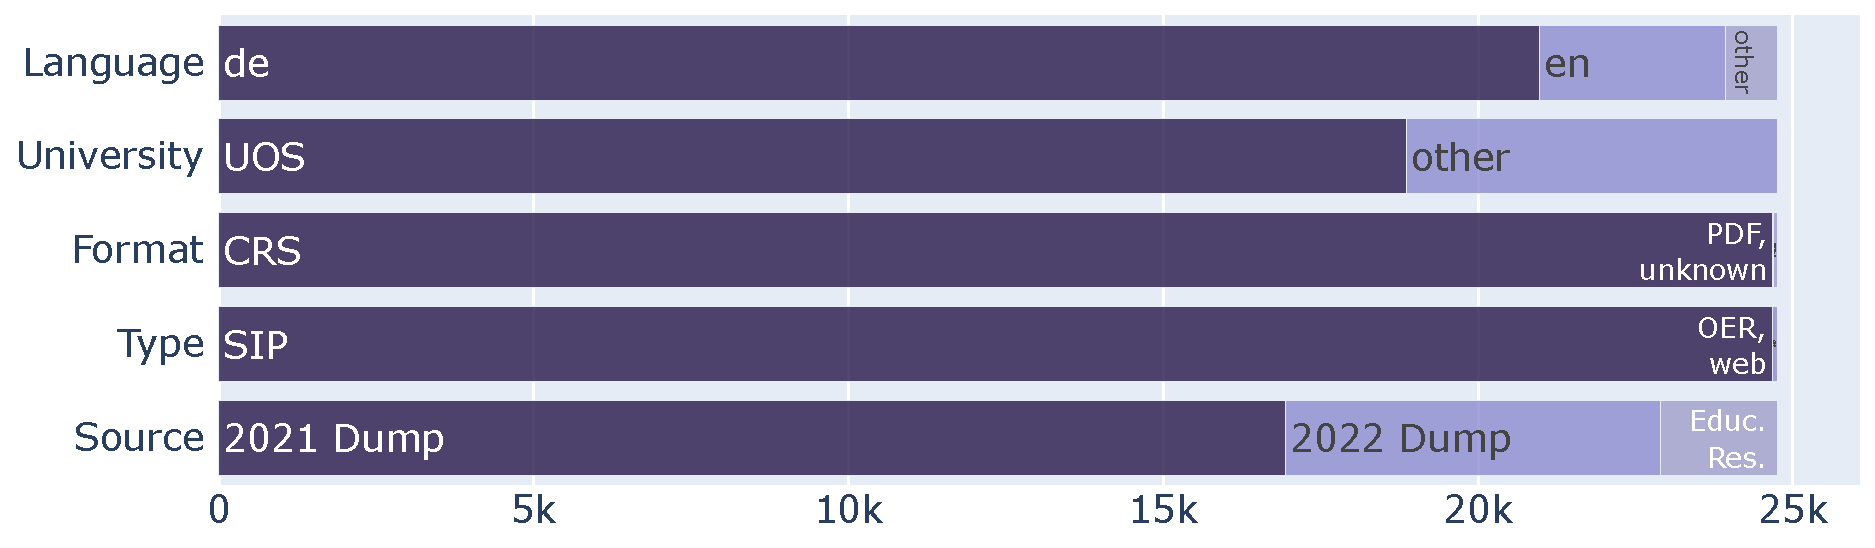
\includegraphics[width=1.15\textwidth,center]{graphics/dataset_new/statistics_bars.pdf}
	\caption{Distribution of metadata in the raw Siddata-dataset}
	\label{fig:sid_statistics}
\end{figure}


\begin{figure}[H]
	\centering
	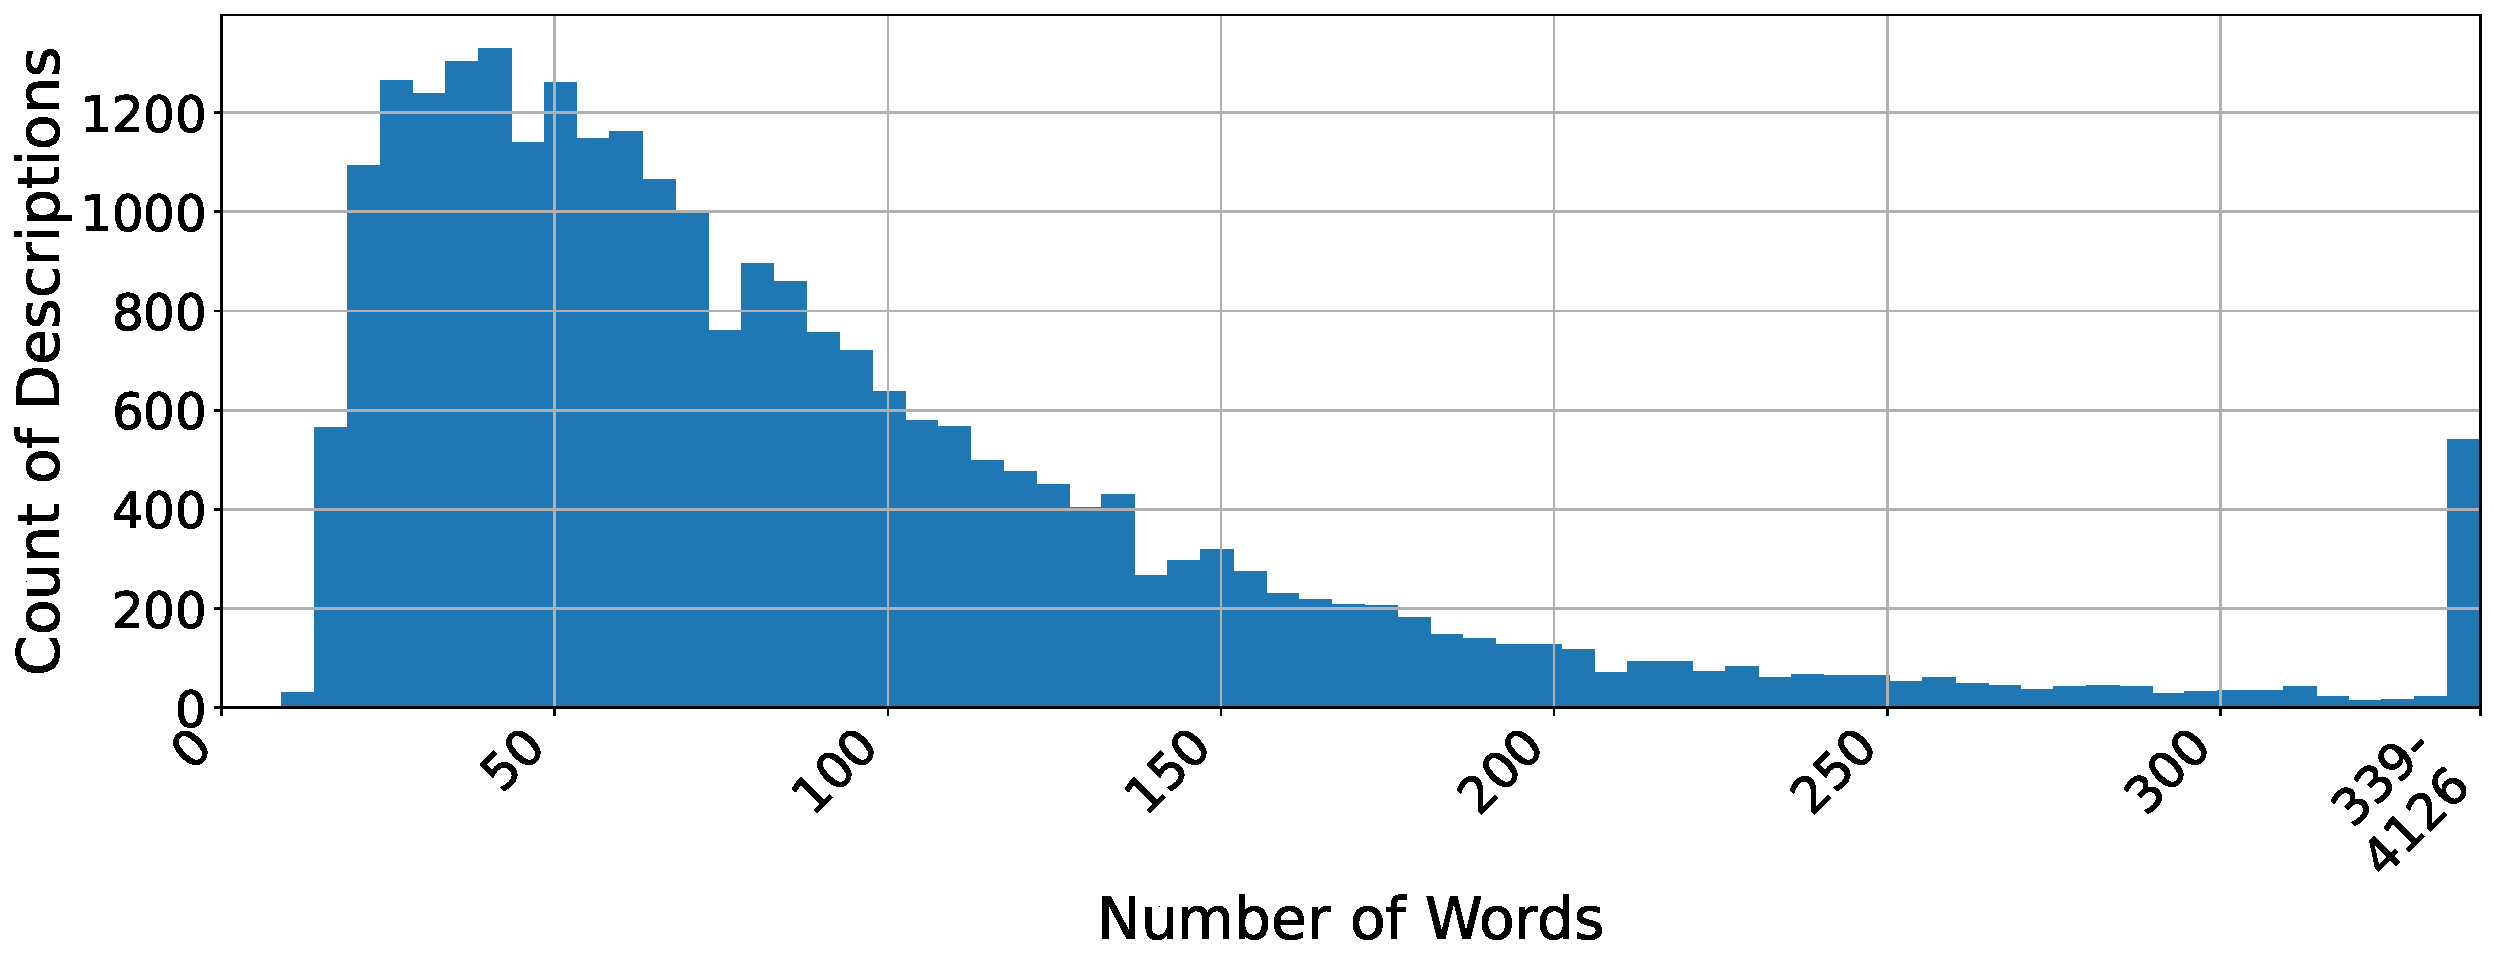
\includegraphics[width=\textwidth]{graphics/dataset_new/words_per_desc.pdf}
	\caption{Distribution of description-lengths of the Siddata-dataset. The rightmost bar represents the longest 2\% of descriptions.}
	\label{fig:sid_wordsperdesc}
\end{figure}

\begin{figure}[H]
	\centering
	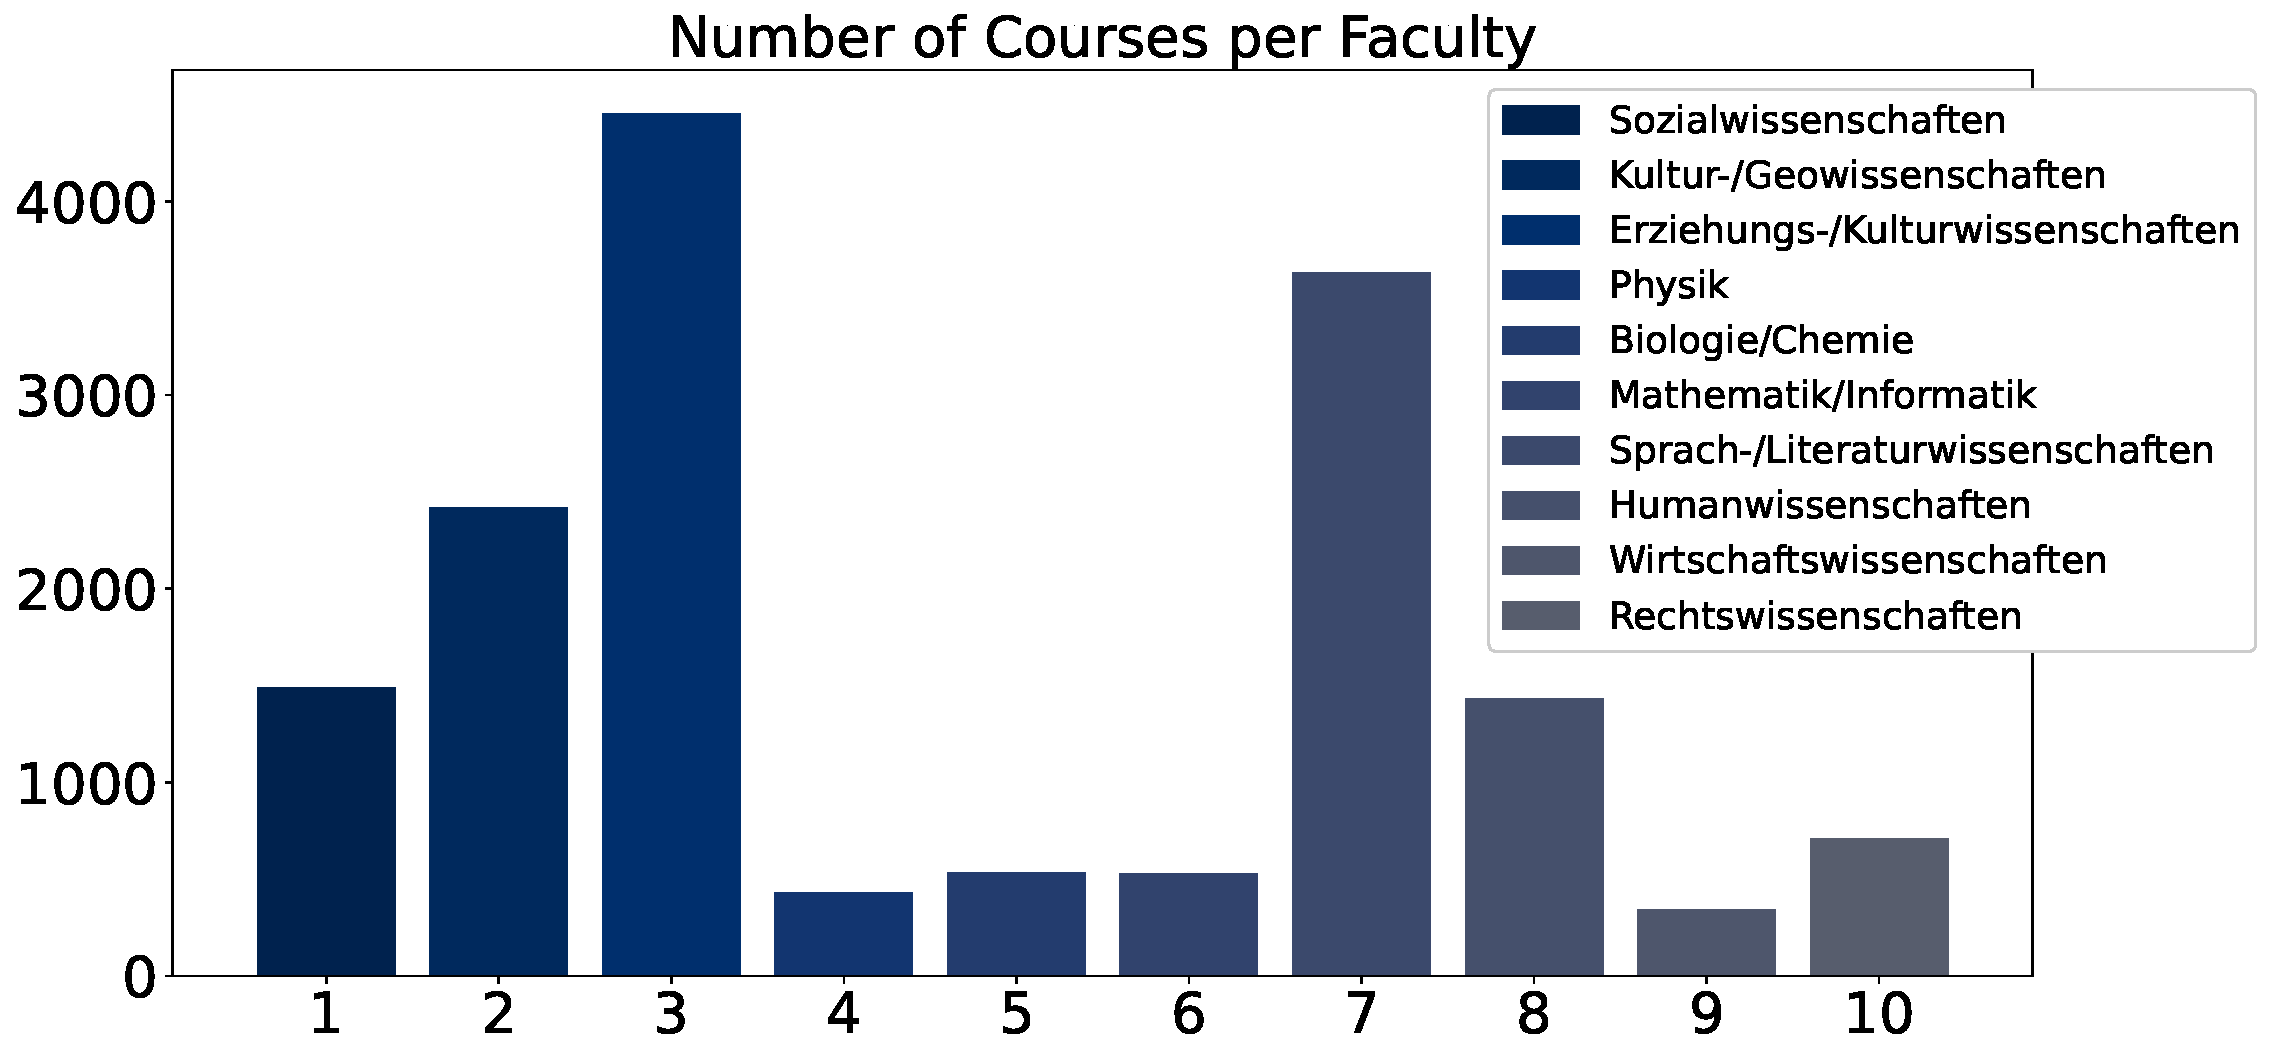
\includegraphics[width=0.95\textwidth]{graphics/dataset_new/courses_per_faculty.pdf}
	\caption{Courses per Faculty}
	\label{fig:courses_per_faculty}
\end{figure}


\includeMD{pandoc_generated_latex/3_0_1_datasets_siddata}

\todoparagraph{Ref auf die Jupyter-plots, wie der sunburst-plot!}


\subsection{Place-Types}
\label{sec:dataset_placetypes}


\begin{figure}[H]
	\centering
	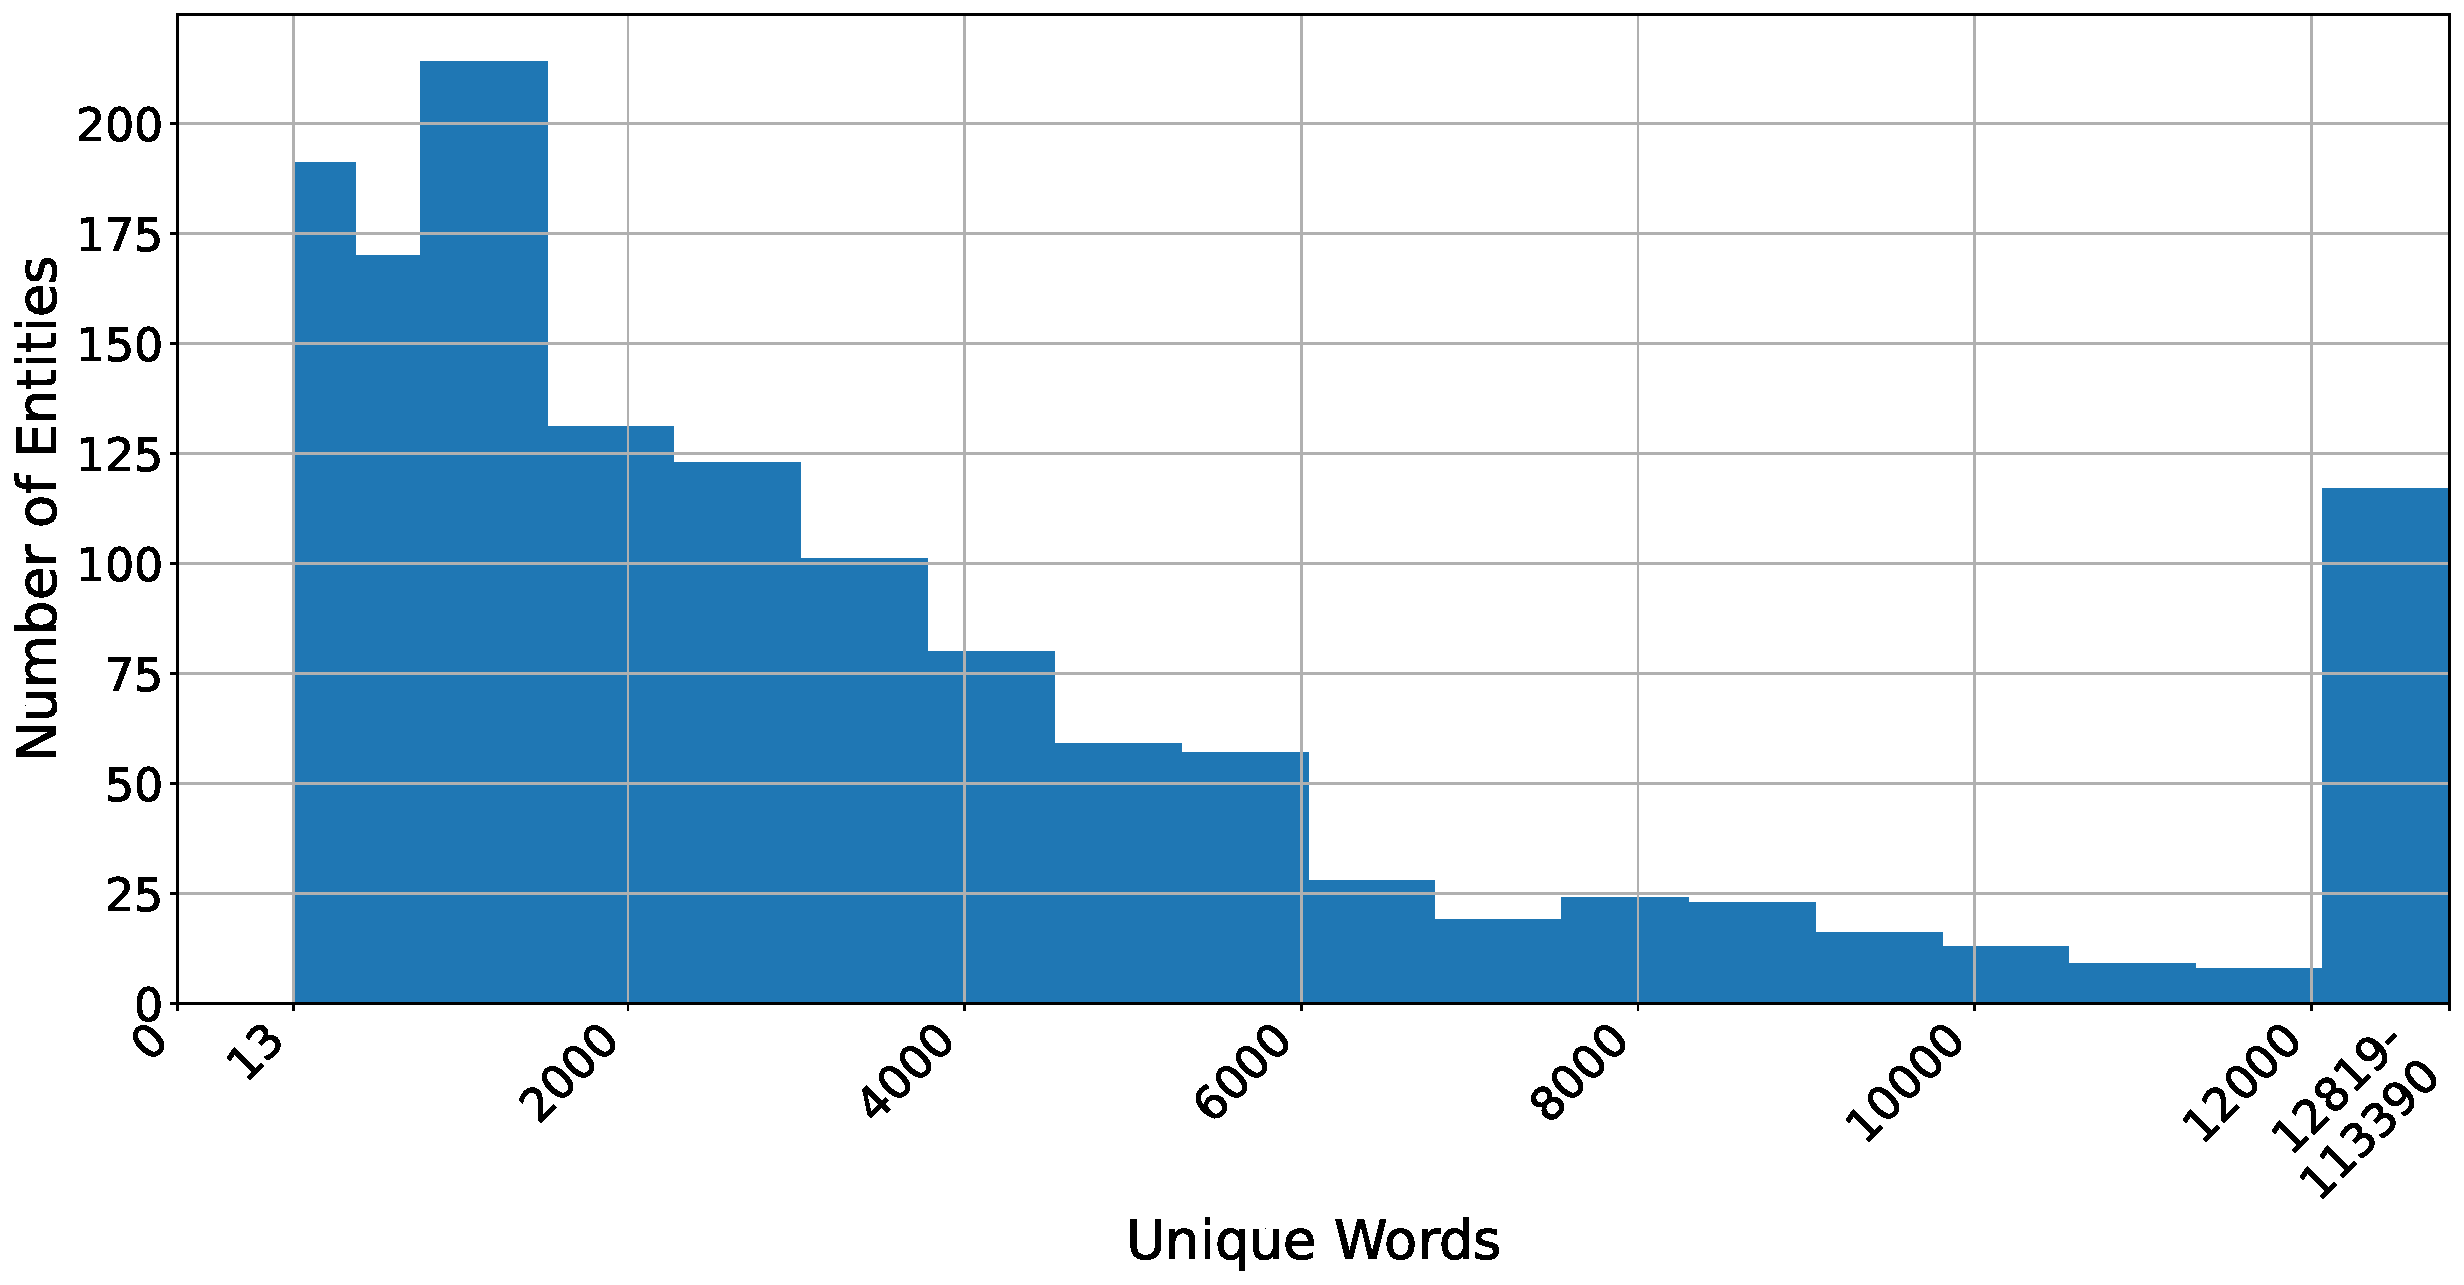
\includegraphics[width=0.8\textwidth]{graphics/figures/placetypes_dist_unique.pdf}
	\caption{Distribution of unique words per entity for the place-types dataset.}
	\label{fig:placetypes_dist_unique}
\end{figure}




Because the SIDDATA-dataset differs in many regards from the datasets used in \mainalgos, %AS stated above (in siddta-section, in the first part of datasecs-section, in workflow-section, ...)
it does make sense to compare the results of the given pipeline on that dataset to the results of \mainalgos. To be able to compare the results achieved here with theirs, one of the datasets used by all of their papers was considered as well. Comparing on a original dataset also has the benefit of allowing to sanity-check if the implenetation is correct. If the performance achieved on this dataset is comparable to the performances of \mainalgos whereas the peformance for the SIDDATA-dataset is considerably worse, there is strong indication that the quality or quantity of the dataset is worse, suboptimal results on this one however would give indication that suboptimal results are the result of a faulty implementation.

There are two datasets used by all three authors: place-types and movie-reviews (see \autoref{tab:all_datasets}). Both of the datasets are available in preprocessed form\footnote{\url{https://www.cs.cf.ac.uk/semanticspaces/}} \cite{Derrac2015}. It was originally planned to use both of the datasets as basis for comparison, however unfortunately it is impossible to recover the form of it as originally used by \textcite{Derrac2015}: The original texts of the reviews are not available, but only their respective bag-of-1-grams (\glsentrylong{bow}) - even though the authors explicitly state that they worked with variable-length-n-grams. Even though the provided list of \glspl{cand} contains \glspl{ngram}, it is impossible to recover which of the \glspl{entity} contained it. While the algorithm can still be run only for the 1-grams, the results are not comparable with the original ones anymore\footnote{As all of the \mainalgos share an author, it is assumed that \cite{Alshaikh2020,Ager2018} had access to the full version of the dataset and did not share the stated problem.}.

\includeMD{pandoc_generated_latex/3_0_2_datasets_placetypes}

\subsection{Other Datasets}


\includeMD{pandoc_generated_latex/3_0_3_datasets_other}

\section{Algorithm}


Let us finally go into detail about the main algorithm. The implementation of this thesis replicates and extends the algorithm proposed by \textcite{Derrac2015} with some novel contributions to deal with the given dataset. Further, some improvements from the works of \textcite{Ager2018} and \textcite{Alshaikh2020} are incorporated, who also replicated and improved the original algorithm and published together with Prof. Steven Schokaert. According to our evaluation of the field, these two papers provide some useful improvements in several aspects, as they apply the algorithm to different datasets, suggest more straight-forward ways of evaluating their performance, and help in understanding important concepts. That we are focusing on only those three papers should by no means imply that they are the only ones that were considered and influcenced this implementation,\footnote{See \autoref{sec:otherwork}} however in contrast to the other pertinent literature these two works do not substantially divert from the algorithm's core principles.
% see \autoref{sec:otherwork} - \cite{VISR12} and their tag genome, the fact that the algorithm detailed here is basically only one step in \cite{Alshaikh2019}, Gärdenfors himself suggested that one may use self-organizing maps instead of classical AI/NLP algorithms.

It is important to keep in mind that the algorithm is no rigid monolith but modularly consists of several components, such as \textit{dimensionality reduction}. Many of these components do not require specific algorithms, and \mainalgos also experiment with different components. The exact system for these components may be exchanged, and in the following these exchangeable algorithms are also referred to as hyperparameters. Note further that while this thesis mostly replicates the work of \textcite{Derrac2015}, the following will describe the algorithm as implemented here, which differs in some details from the original work. For the sake of clarity, very specific implementation details will be left out in the following description, as however reproducibility is an important aim for us, implementation details are available in Appendix~\ref{AppendixB} and linked where relevant. %\todoparagraph{Further, there is a table that compares the implementations here and in mainalgos, as well as another table what-configs-are-available where, the config-yamls and a section on what-other-things-could-one-have-done-hereandthere.}

\subsection*{Core Algorithm}

%\todoparagraph{The following explanation assumes that we accept some things as given. For now we'll do that, but we will later revisit and critically question many of these assumptions!}

% The core idea of the algorithm is to unsupervisedly find a a set of features which can be modelled as directions for a vector-space representation of the respetive entities.
The main goal of the algorithm is to unsupervisedly use text-corpora associated with the considered \glspl{entity}\footnote{From now on, the term \textit{\glspl{entity}} refers to the sample described by one text from the corpus (description, concatenated reviews, ...) from a certain domain. The corpus accordingly defines the domain: educational resources, movies, ...} to embed these into a vector-space where the axes correspond to human concepts/properties.\footnote{\textit{Concepts} and \textit{Properties} explicitly refer to what is defined in Criterions C and P, see \ref{sec:csdefinition}} This is referred to as \textit{feature-based} representation: A high-dimensional vector that numerically encodes the degree (\textit{protoypicality}) to which the entity corresponds to a number of appropriate dimensions. This is generally referred to as Conceptual Space and can be used as basis for explainable reasoning.

The general idea to achieve that is as follows: First, the entities are embedded as fixed-dimensional vectors. To allow for the types of reasoning from \autoref{sec:cs_reasoning}, it is embedded into metric spaces where the concepts of direction and distance are well-defined. \gencite{Derrac2015} original algorithm uses MDS (see \ref{sec:mds}) for this matter, which enforces metric distances. \cite{Ager2018,Alshaikh2020} both soften this requirement and also use document embedding techniques such as \gls{doc2vec} and averaged GloVe \cite{pennington2014glove} embeddings.

Additionally, words or phrases from the text are extracted as candidates for the names of the semantic dimensions. The underlying assumption is that \q{words describing semantically meaningful features can be identified by learning for each candidate word $w$ a linear classifier which separates the embeddings of entities that have $w$ in their description from the others} \cite[3574]{Alshaikh2020}: The better the performance of that classifier according to a chosen metric, the more evidence there is that $w$ describes a semantically meaningful feature. 
% * from Alshaikh2020: "Their core assumption is that words describing semantically meaningful features can be identified by learning for each candi- date word w a linear classifier which separates the embeddings of entities that have w in their description from the others. The performance of the classifier for w then tells us to what extent w describes a semantically meaningful feature"
In a final step, the candidate-words are clustered according to their similarity to find a fixed set of \emph{semantic directions}. A representative term for the directions is selected as dimension name, and the entities are re-embedded into a new space comprised of these dimensions, where the individual vector-components correspond to the ranking of an entity with respect to these dimensions.

The rest of this section goes into further detail for each of the individual algorithm components. \removeMe{An overview of which of the considered literature supports each components is given in \autoref{tab:compared_algos}.} Further, configuration files to enable exactly the respective components of the papers \mainalgos for the codebase of this thesis are listed in \aref{ap:yamls_for_origalgos}.

\todoparagraph{but before that, ager and alshaikh}

\removeMe{
\subsection{Regarding ager and alshaikh}

\todoparagraph{describe shortly what the improvements from [2,3] were}

\todoparagraph{Dass die den Zwischenschritt mit dem ganzen geeometric reasoning auf dem interim space nicht machen und DESWEGEN die requirement mit MDS soften konnen}

In principle Derrac2015, but with some components from Ager2018 and Alshaikh2020 as well as some own stuff. We will testi some claims or nonclaims of \mainalgos, bspw nutzen sie immer PPMI ohne je tf-idf zu testen. Also of course different nature of the dataset - their "how does this dimension correspond to the count in the reviews" doesn't make sense (their success-metric for the SVM is tailored to the one property, so we expect that one to be worse). We will elaborate on different ways to deal with that later.
}

\subsection{Algorithm Steps}
\label{sec:algorithm_steps}

% The core idea of the algorithm is to (unsupervised, data-driven) find a a set of features which can be modelled as directions for a vector-space representation of the respective entities. For that, the steps are:

This section describes the steps how to create an interpretable vector-space from the text corpus in detail. For that, we will explicitly elaborate on the parameter choices that branch up at every step for this specific implementation. %Note that absolutely is a combinatorical explosion it is impossible to try out all. %Further, this is about how this specific implementation does it, which may differ in some details from \mainalgos.

\label{sec:algorithmsteps}
\begin{enumerate}
	\item[\saveref{sec:algo_preproc}{1.}] \textbf{Preprocess} the corpus with default techniques and create a \textit{Bag-of-ngrams representation} (\ref{sec:techniques:bow}) of the texts.
	\item[\saveref{sec:extract_cands}{2.}] \textbf{Extract Candidate Feature Names} from words/\glspl{ngram} of the corpus.
	\item[\saveref{sec:generate_vectorspaces}{3.}] \textbf{Embed all Entities} into a fixed-dimensional vector space with demanded properties that captures the respective semantics.
	\item[\saveref{sec:svm_filter_cands}{4.}] \textbf{Filter Candiate Features} by training a linear classifier for each candidate that seperates the vector representations of the entities that contain the term from those that do not. If a specified metric for this classifier is sufficiently high, assume that the candidate term captures a \textit{salient} feature - its direction is then characterized by the orthogonal of the classifier's separatrix.
	\item[\saveref{sec:algo:cluster}{5.}] \textbf{Cluster/Merge the candidates} and calculate the feature direction for each cluster from its components, and (optionally) find a representative cluster-name.
	\item[\saveref{sec:algo:postprocess}{6.}] (optionally) \textbf{Post-process} the candidate-clusters.
	\item[\saveref{sec:algo:reembed}{7.}] \textbf{Re-embed the entities} into a space of semantic directions by calculating their distance to each of the feature direction separatrices.	
\end{enumerate}

This techniques first embeds the collection of texts into a  vector space, to afterwards extract important features from this space using linear classifiers. The second step is an original idea of \cite{Derrac2015}, however creating vector space embeddings from texts is a very popular technique, used for many tasks in \gls{nlp} \cite{Mikolov:Regularities,Mikolov2013a,Guo,Lowe,Turney2010}. This implementation relies on classical creation of the \gls{vsm}, for which the general creation process was explained in \autoref{sec:vsm_construction}. The steps \textit{Build the Frequency Matrix}, \textit{Transform Raw Frequency Counts} and \textit{Smooth the Frequency Matrix} are squashed into the preprocessing and embedding of entities. When \textit{extracing candidate features}, their frequencies must additionally be quantified - which may differ from the quantification when \textit{embedding all entities}.

An explicit and simple implementation compliant with each step could be a simple word tokenization and count to generate a bag-of-words (step 1) where each sufficiently frequent word is used as candidate (step 2). A \gls{dissimmat} of the individual \gls{bow}-vectors is compressed using MDS (step 3). A \gls{svm} calculates the accuracy for each candidate (step 4), and k-means-clustering on the 500 top-scoring terms subsequently creates 100 clusters and averages their directions (step 5). The distance to each of the hyperplanes is calculated (step 6), yielding new space for the entities. The sequence of steps is also given as pseudocode in \autoref{ap:algorithm_pseudo}. 
 
 The distinction of steps is not always this rigid: Instead of creating a dissimilarity matrix followed by dimensionality reduction, \cite{Ager2018,Alshaikh2020} use neural word or document embeddings.\footnote{see \autoref{sec:embeddings}} %Instead of extracing candidates from corpus tokens and training a linear classifier for each of them and use their orthogonal as direction, techniques such as LSA or LDA can be employed to find topic vectors directly. 
 We will come back to other ideas ideas when discussing future research opportunities (\autoref{sec:futurework}) by listing what other ways of fulfilling each respective step could have been considered.

\autoref{fig:dependency_graph} shows an automatically exported dependency-graph, displaying the individual steps of the algorithm as done in the accompaning code, also showing where selected important parameters are first used. As explained in \autoref{sec:architecture}, the modularity of the provided architecture allows individual components to be exchanged as needed and run in parallel.


\begin{figure}[h]
	\begin{center}
	  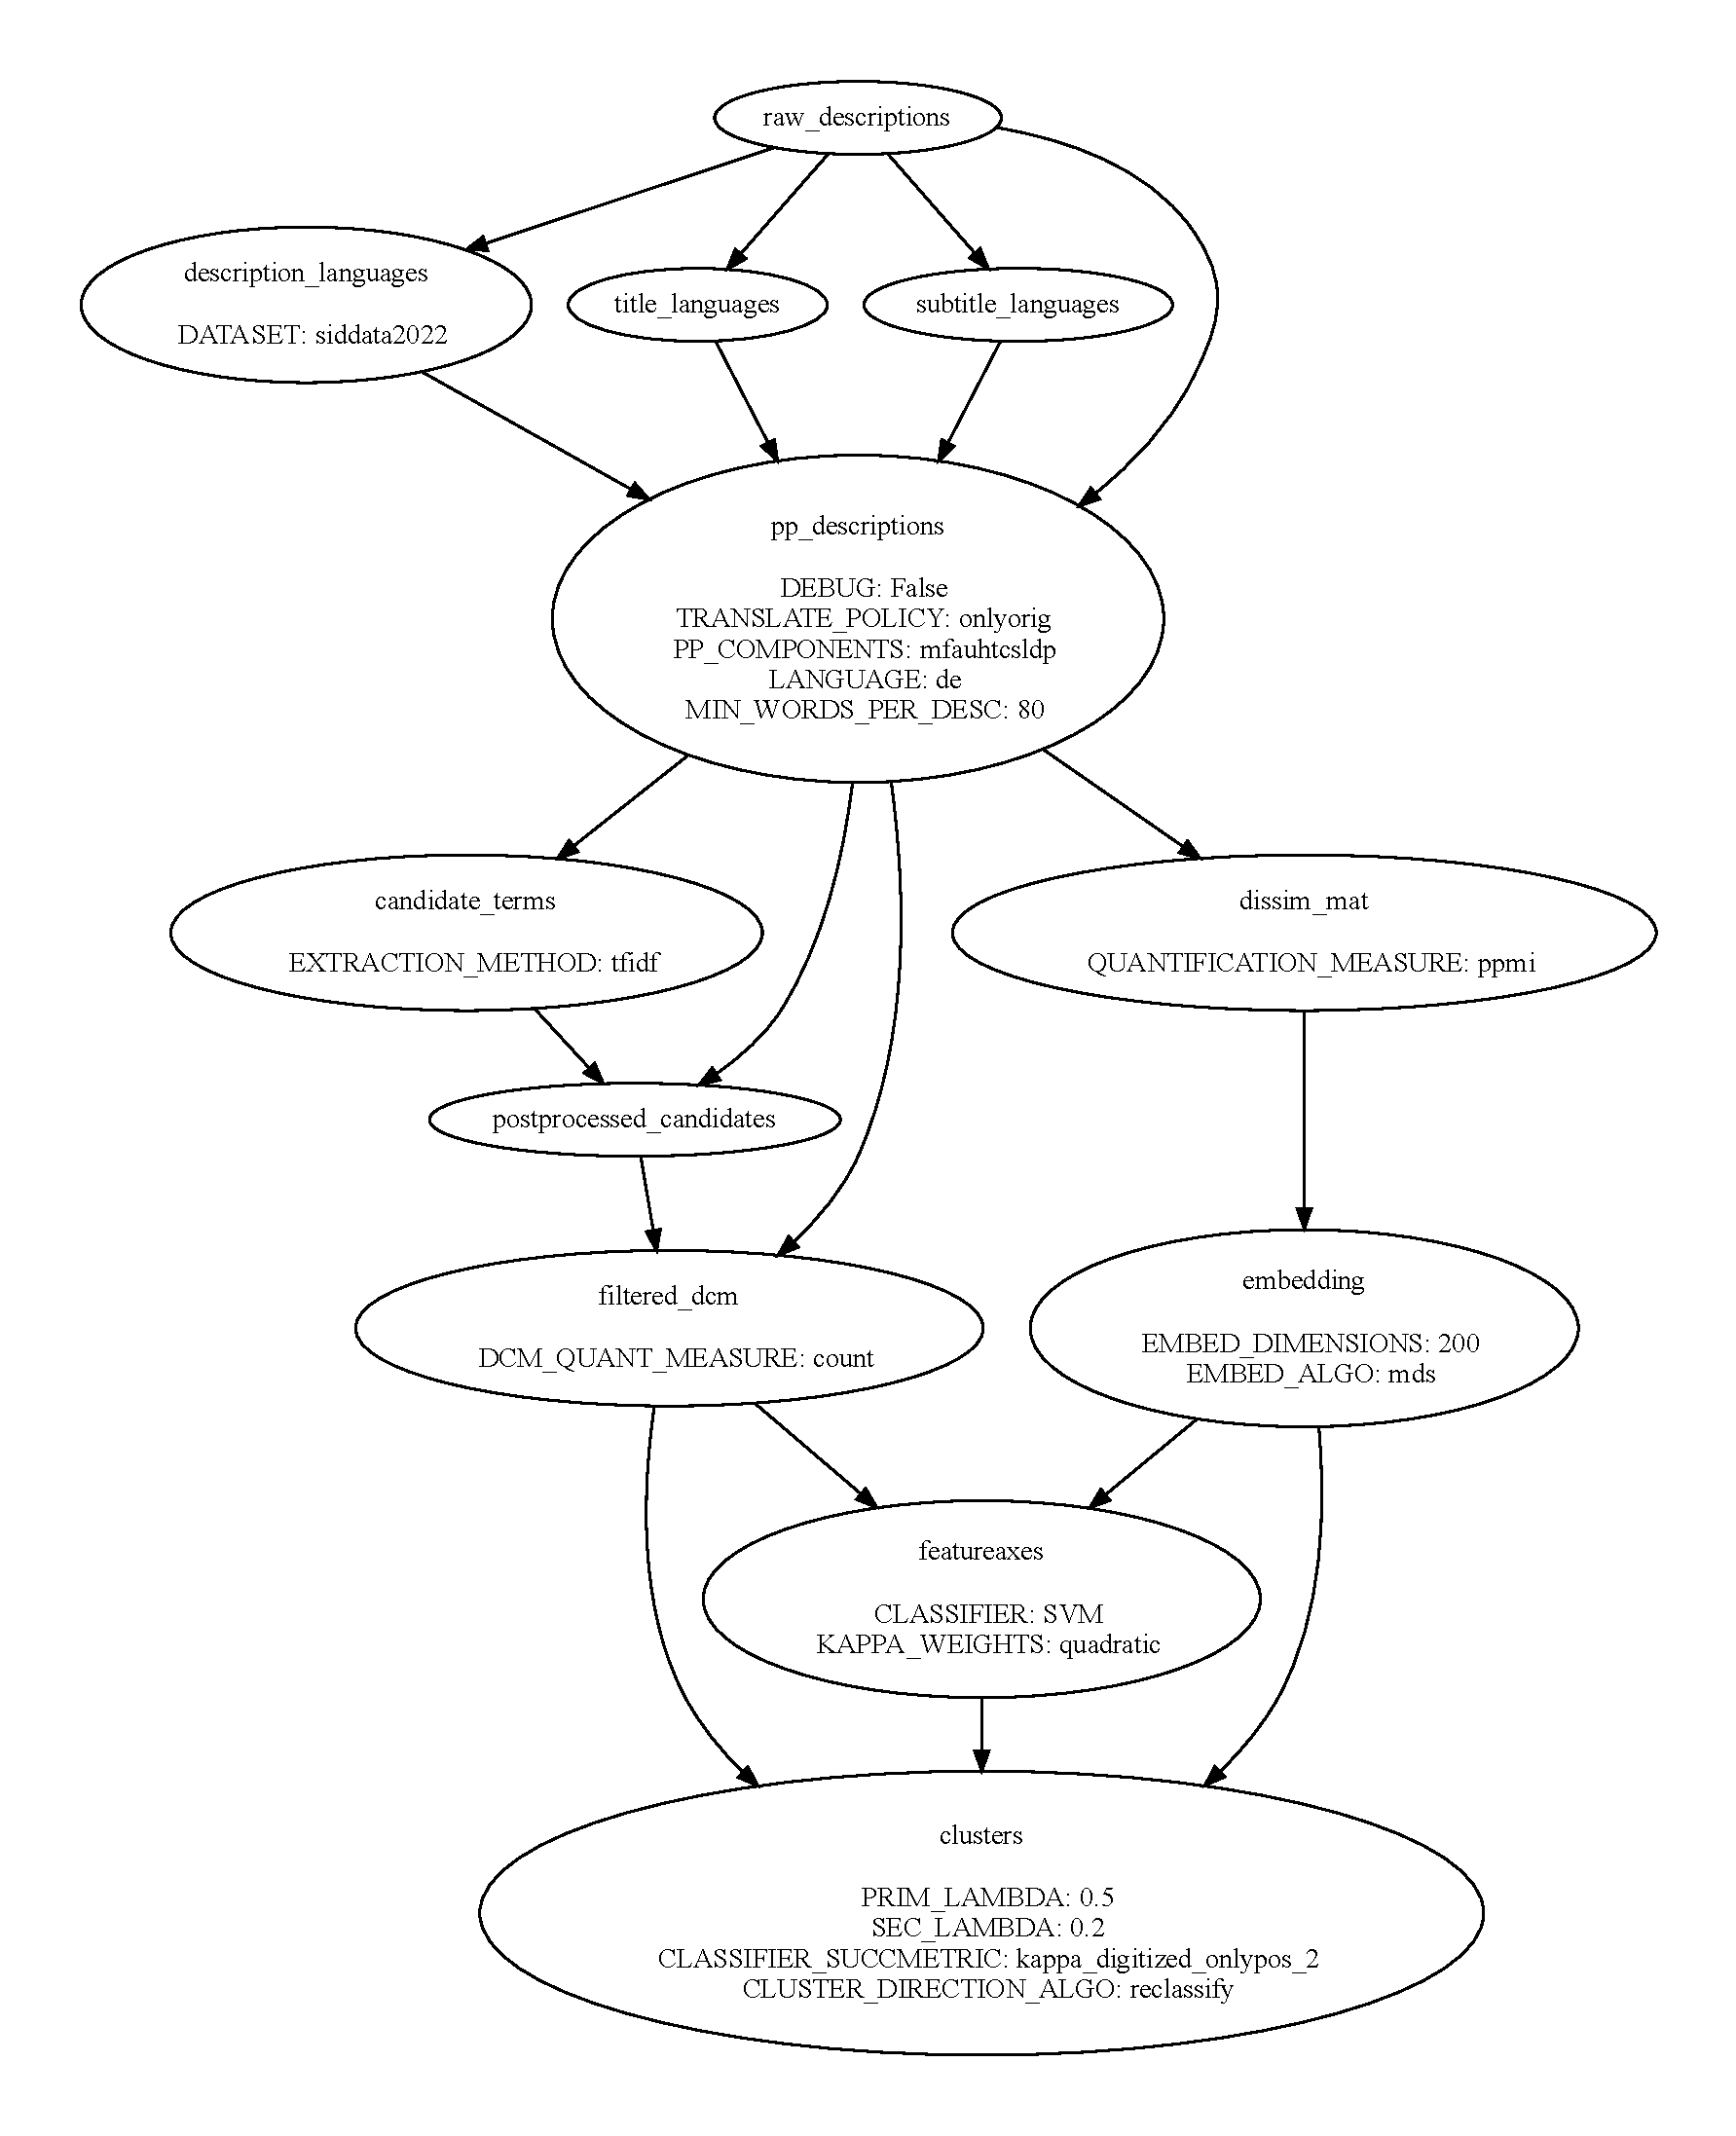
\includegraphics[width=0.9\textwidth]{dependency_graph.pdf}
	  \caption[Dependency-graph of the implementation]{Dependency-graph of the implementation, displaying the individual steps of the algorithm as well as their dependencies and where selected important parameters are first used. \todoparagraph{Generated using command XYZ}}
	  \label{fig:dependency_graph}
	\end{center}
\end{figure}


\subsubsection{Preprocessing\arrowref{sec:algorithmsteps}}

\label{sec:algo_preproc}

Before looking at the steps in turn, it should be noted that even the preprocessing does not work on completely raw data, but on curated and processed corpora. This processing is however not considered part of the algorithm, as it is very specific to the respective datasets and manual dataset exploration, tweaking settings such that they are best for each corpus separately. The preprocessing for the Siddata-dataset is described in \autoref{sec:dataset_siddata} and its implementation is done in separate Jupyter Notebooks.\footnote{Such as \url{https://github.com/cstenkamp/derive_conceptualspaces/blob/main/notebooks/create_datasets/Preprocess_Siddata2022.ipynb}} In the considered literature, the preprocessing is not considered part of the algorithm at all. Their implementations start from already fully processed datasets available as bag-of-words, each separately processed. Details of their individual processing per dataset is listed in \autoref{tab:all_datasets}. By incorporating the preprocessing into the pipeline, this work aims to increase adaptability and reproducibility, and also allows to experiment with different techniques such as translation or lemmatization or how duplicate entities with different associated texts are merged.
% In course-descriptions, I want some parts of the pre-preprocessing be part of the pipeline, like how we merge descriptions of different iterations of the same course that overlap to a high degree (sentwise-merge vs relative-term-frequencies)


A common prerequisit for NLP algorithms is to pre-process the text corpus. The preprocessing itself consists of multiple independent components chained after each other. Which components are necessary also depends on the processed dataset - as for example the \emph{placetypes}-dataset consists of a collection of \textit{tags} instead of full sentences, tokenising sentences or removing \glspl{stopword} becomes irrelevant. Other datasets may require additional cleaning or are already available in preprocessed form.

\paragraph{Translation} As the main considered dataset of university-courses is highly multilingual (see \autoref{fig:sid_statistics}), one of the first questions that needs to be addressed is how entities of different languages are handled. The algorithm consists of classical language processing algorithms such as comparing \gls{bow} representation of the entities, which means that the same text in two different languages may result in maximally different representations (see \autoref{sec:techniques:bow}). Because of this, before any other processing, the languages of each entity is checked, such that those of languages other than the demanded may be either translated, left out or used anyway. For details about the translation, it is referred to Appendix \ref{ap:translating}.\footnote{It should be noted that professional automatic translation is costly and thus not all texts are available in all languages.}

\paragraph{Components} The following components are developed for the preprocessing, every one of which can be individually enabled or disabled:

\begin{itemize}
	\item Prepend title and/or subtitle to the entities' associated text \itemtext{useful for the Siddata-Dataset, as the titles are often quite long and more descriptive than their descriptions}
	\item Remove HTML-Tags from texts 
	\itemtext{useful for the Siddata-dataset, as it includes descriptions for \glspl{mooc} which are crawled from websites and often contain such}
	\item Tokenise sentences 
	\itemtext{such that \glspl{ngram} across sentences are not considered}
	\item Lower-case all words
	\itemtext{reduces the amount of individual words and ensures that words at the beginning of sentences are mapped correctly}
	\item Remove stop-words / frequent phrases
	\item Tokenise words
	\itemtext{means splitting at the word-boundary, resulting in a list of words. Order must be kept in case n-grams are to be extracted.}
	\item \Gls{lemma}tize words
	\item Remove diacritics
	\itemtext{\emph{Diacritics} are glyphs added to basic letters, such as accents or German \emph{Umlaute}. Removing them converts for example the letter \emph{ä} to an \emph{a}}
	\item Remove punctuation 
\end{itemize}

The above can be done either be done with proprietary code for all of these steps,\footnote{Mostly relying on the python package \emph{nltk} \cite{bird2009natural}} or using \codeother{sklearn}\footnote{\url{https://scikit-learn.org/stable/}}s \codeother{CountVectorizer} (which is faster, but less configurable), as \cite{Ager2018} claim to have done.

\paragraph{On Stop-Words}
Removing stop-words from the texts is useful because it makes the resulting frequency more compact and thus less computationally intensive, and stop-words generally have very discriminative power, meaning their occurence among the entities is arbitrary, just making hte emeddings more noisy (cf. \autoref{sec:word_count_techniques}). There are however reasons to not remove them: Two words that are considered stop-words may posess relevant semantic content (such as a \textsc{Fällt aus} in a course title), and stopwordslists are often incomplete and of low quality \cite{nothman-etal-2018-stop}. For these reasons it is also possible to instead remove \glspl{ngram} that exceeded a certain frequency (\gls{df}).

\paragraph{On Lemmatization}
The languages most prevalent in the considered datasets are considered \textit{agglomerative}, which means word stems are changed by the addition of affixes and suffixes. Consequently, the same word may be present in multiple different forms, which modelled as completely dissimilar vectors in the present \glspl{bow}-approach. Lemmatization is the process of mapping different forms of these words onto the same stem. Considering that the Siddata-dataset consists of far fewer words than the others, this has important implications. For the german descriptions, this implementation relies on the \textit{HanTa} lemmatizer \cite{Wartena2020}.\footnote{\url{https://textmining.wp.hs-hannover.de/Preprocessing.html\#Lemmatisierung}}

The result of this step is a bag-of-ngrams representation for each entity (see \autoref{sec:techniques:bow}).


\subsubsection{Extract Candidates\arrowref{sec:algorithmsteps}}
\label{sec:extract_cands}
% Section 4.2.1 of Derrac2015

The final result of the algorithm is a metric space in which the individual dimensions (\emph{\glspl{feature}}/\emph{interpretable directions}) correspond to natural-language concepts and attributes. The candidates for these features are verbatim phrases extracted from the text-corpus of the \glspl{entity}, which are subsequently filtered and merged as necessary.

In \gencite{Derrac2015} work, the selection of phrases to be extracted depends on the dataset: For placetypes-dataset, all sufficiently frequent\footnote{\label{fnote:cand_thresholds}The respective thresholds are listed in \autoref{tab:all_datasets} as ``candidate word threshold''.} 1-grams\footnote{Note that in the case of the placetypes dataset, a 1-gram corresponds to all merged words of a tag.} were considered. For the other two datasets, they applied a \gls{pos}-tagger that extracted all sufficiently frequent\footnoteref{fnote:cand_thresholds} \textbf{adjectives, nouns, adjective phrases} and \textbf{noun phrases}, assuming that adjectives would correspond to gradual properties (\eg \textit{violent, funny}) and nouns to topics (\eg the \textit{genre}) \cite[Sec. 4.2.1]{Derrac2015}. Also, the authors ensured that the number of extracted candidates for both datasets is roughly equal, getting around 20\,000 candidates for movies and placetypes.

% Their method depended on the dataset - as their placetypes-dataset was just a collection of tags and the number of tags with term-freq >= XYZ (docfreq>2?! hä?) corresponded to their desired number of candidates anyway (around 22k), they just took all of these as candidates. For their movie-reviews-dataset, they considered all nouns, adjectives, nounphrases 	and adjective-phrases as detected by a POS-tagger. Doing something similar in the scope of this thesis led to suboptimal results, which is why alternative methods were developed
For this step, the implementation of this thesis differs from the original algorithm, as both taking all words as candidate and running a \gls{pos}-tagger led to suboptimal results in previous experiments, which indicated that the robustness of the algorithm is increased if less candidates are considered in earlier steps. \todoparagraph{This will be further argued and elaborated in the discussion.} To ensure comparability to these works however, in the case of the placetypes-dataset the original method of taking all words with a term-frequency of at least 50 was used. Similar techniques for the Siddata-dataset were also considered, but in constrast to the placetypes-dataset it is also important to consider various-length n-grams. 

% \todoparagraph{thing is I have less words but the algorithm seems to profit from less words as that makes it more robust}
% I would however argue that the difference here doesn't make a relevant difference 

In our implementation the candidate-extraction is split into four subsequently excecuted substeps, because depending on the algorithm used to extract the candidates the runtime of the individual components is comparably long and some settings are only relevant in later substeps. The steps are:
\begin{itemize}
	\item Extracting Candidate Terms
	\item Postprocessing the Candidates
	\item Creating the \gls{doctermmat} for the candidates and applying a \gls{quant}
\end{itemize}

As visualized in \autoref{fig:dependency_graph}, these substeps only depend on the preprocessed descriptions, which means they can be run in parallel to the creation of the embedding if \eg running on compute clusters.

% This can be done either based on the frequency (meaning all terms with a minimal term-frequency), based on some notion of *importance* (based on scores like tf-idf or ppmi), or by more complex means of figuring out *important* keywords and keyphrases. An example of the latter would be KeyBERT
Three main techniques are implemented to extract candidates from the text-corpus. Irrespective of the algorithm, only words with a sufficiently high \gls{df} are extracted, which is important to ensure that the classifier that determines its meaningfulness has enough samples in both clases. This means that the minimal freqeuncy can be calculated from the dataset size: In \cite{Derrac2015}, the minimal frequency for the movies-dataset with 15\,000 entities was only 100, meaning that the algorithm even works if only 0.6\% of samples are in the positive class. 


\begin{description}
	\item[By frequency:] consider all phrases that exceed a specified document-frequency (like \cite{Derrac2015}).
	\item[By a \gls{quant}:] consider all phrases that are prominent by some notion of \textit{importance} , such as the \gls{ppmi} or \gls{tf-idf}-score. Note that the respective scores depend on the combination of document and term, such that candidates may be extracted for some documents. Of course, all their occurences are considered in the creation of the frequncy matrix.
	\item[Using \emph{KeyBERT}\cite{grootendorst2020keybert}:] consider phrases whose BERT-embedding \cite{Devlin2019} is most similar to the text they are in. 
\end{description}

Using KeyBERT results in candidate terms that are most appealing in qualitative inspection, however it is also most computational demanding, techniques and requires substantial amounts of post-processing for the resulting phrases. More details on KeyBERT and how it is incorporated into the algorithm are given in the implementation are given in Appendix~\ref{ap:details_keybert}

Finally, a \gls{doctermmat} is created from the postprocessed candidates, containing the frequency for each candidate-phrase in each entity. The creation of this frequency matrix mirrors the process described in \autoref{sec:vsm_construction}, however only for the extracted words. After filtering this matrix to ensure that only candidates with a minimal \gls{df} or \textit{stf} are considered, a quantification is applied as described in \autoref{sec:word_count_techniques}. Available Quantifications include raw count, binarization\footnote{meaning all counts are either one or zero. According to \textcite{Alshaikh2020} this improves performance, however we could not confirm this.}, tf-idf or PPMI. We expect that expressing the relation of terms and documents by something else than the raw count will prove especailly useful for the Siddata-dataset: As it does not consist of concatenated reviews but short descriptions, each individual word will only occur a few times per description. Because of that, a \gls{rank} induced from the count will be not very meaningful when later comparing it to the ranking induced by the classifier.

\subsubsection{Generating Vector Space Embeddings\arrowref{sec:algorithmsteps}}
\label{sec:generate_vectorspaces}

In this step, the individual \glspl{entity} are embedded into a fixed-dimensional vector space, making up a \emph{frequency matrix}.\footnote{The previous step already created a frequency matrix that encodes the relevance of a candidate-phrase for each entity- this is a spearate one that later serves to encode each document as a vector} Neither this nor the frequency matrix from the previous step will used to finally calculate similarities on, but both are interim results to get the dimensions necessary for these similarities.

% Importantly, while this matrix is a \gls{doctermmat}, it is only an interim result in the algorithm and the calculation of distances and directions will be done on another matrix from a later step. %This is where our pipeline starts to diverge from what the pipeline specified in \nameparanref{sec:vsm_construction}.  in the previous step, and in this step we create another one that encodes each document as a vector. 

Embedding words, \glspl{ngram}/phrases or other tokens, as depicted by \cite{Turney2010,Lowe}, generally involves counting the token frequencies, transforming them to get relative frequencies, and performing dimensionality reduction on the resulting matrix.

So far (step 1), we have counted the token frequencies. \textcite{Derrac2015} argued that this space must be Euclidean, such that geometric/algebraic solutions correspond to commonsense reasoning tasks (see \autoref{sec:reasoning}). Another requirement is that the number of dimensions is be chosen as hyperparameter to the algorithm to be able to find a compromise between compression and expressive power. Because of these two requirements, they selected \gls{mds} for dimensionality reduction.

As stated in \autoref{sec:mds}, \gls{mds} calculcates a Euclidean \gls{vsm} from a set of pairwise distances. This means that the algorithm first creates a \textit{Dissimilarity Matrix} that encodes the distance between all pairs of entities (represented as Bag-of-ngrams representation), from which subsequently the final embedding is generated. 

In this implementation, the dissimilarity matrix is created using distance metrics for the quantified bags-of-ngrams of the respective entities. Note that this quantifiation does not need to be the same one as the one used for quantifying the relatedness of the extracted candidates and the documents.\footnote{As will be shown in the result, doing so sometimes even outperformed other configurations.}

\paragraph{Document embeddings}
If the strict requirement for a metric space is dropped however, many different algorithms may instead be used at this point - not only different dimensionality reduction methods for the embedding, but also ones that do not rely on the distance matrix or even the \gls{bow} at all, like document-embedding-techniques such as \gls{doc2vec} \cite{Le2014} (as \eg used by \cite{Alshaikh2020}). This would not require the count of token frequencies followed by a \gls{quant}, but not affect the rest of the algorithm. As, however, document embeddings tend to be created on the basis of \gls{cos}, this will not result in a Euclidean metric. \textcite{Alshaikh2020} experimented with this, however it performed worse than the original algorithm relying on MDS (see \autoref{tab:f1_placetypes_long}), which is why this technique was not futher pursued in this work.

\paragraph{Classical Processing}
The default way of doing it is, however, to create frequency matrix counting the token frequencies of each word of an entity and using a \gls{quant} to transform these raw counts. In this implementation, the \gls{dissimmat} that is required for the MDS-algorithm created on basis of the \emph{normalized angular distances} of the \glspl{bow} of the respective entities, which is relates to the \gls{cos} and is defined by \textcite{Derrac2015} as:

\vspace{-5ex}
\begin{align}
	ang(e_i, e_j) &= \frac{2}{\pi} * \arccos \left( \frac{\vec[m]{v_{e_i}} * \vec[m]{v_{e_j}}} { \lVert \vec[m]{v_{e_i}} \rVert * \lVert \vec[m]{v_{e_j}} \rVert }  \right)  \label{eq:norm_ang_dist} \\
	&= \frac{2}{\pi} * \arccos(1-\cos(\vec[m]{v_{e_i}},\vec[m]{v_{e_j}})) \nonumber
\end{align}

Finally, the dimensionality of the frequency matrix is reduced using the MDS-algorithm described in \autoref{sec:mds}. \cite{Derrac2015} also experiment with the \textit{Isomap} algorithm, which does not yield a Euclidean space but one of geodesic distances. As the results for their implementation are, however, of worse quality than those for MDS, it is not considered further in this work. 

In the publication of \textcite{Derrac2015}, the result of this embedding is used to experiment with the explainable classifiers (discussed in \autoref{sec:reasoning}). Due to the usage of MDS, this space has clearly defined concepts of \textit{betweeness} and \textit{parallesism} between the entities, however it is important to stress that it does not have interpretable dimensions and is, so far, a plain \gls{vsm} as described in \autoref{sec:vsm_construction}. 


\subsubsection{Filter Candidates by Classifier Performance\arrowref{sec:algorithmsteps}}
\label{sec:svm_filter_cands}

This step brings together the entity embeddings and the extracted keyphrases, to finally find semantically meaningful directions in the space the entities are embedded in. For that, classifiers are trained for all previously extracted candidates, each yielding a \textit{Candidate Feature Direction}, which are subsequently filtered to detect those corresponding to semantically meaningful features. The algorithm is executed separately for each candidate term and looks as follows:

All entities are split into two classes: Those that contain the respectively handled candidate term and those that do not. To quantify how well each candidate word captures semantic content of the entities, a linear classifier is trained to separate the embeddings of these two classes. The best example for such a classifier is a \gls{svm} which does not rely on the kernel trick. As visually exemplified in \autoref{fig:3d_hyperplane_ortho}, the result is a hyperplane that best divides the positive from the negative samples. Regardless of the dimensionality of the original space, this hyperplane has a one-dimensional orthogonal vector. Each of the entity-embeddings is subsequently orthogonally projected onto it. The distance of this projection to the plane offset\footnote{The coordinate where it crosses the decision surface} is a scalar that encodes the distance to this decision hyperplane. 

This distance encodes \textit{how much} this point is considered to be protoypical of the respective class by the classifier, for the positive as well as the negative class. Given that the original space is created based on similarity measures of the entities, the \textit{Bag-Words-Hypothesis} (\autoref{sec:bow_hypothesis}) states that similar words should have similar words - meaning maximally dissimilar entities are far apart from positive ones.\footnote{To stick with the example of movies, the assumption is that movies that are maximally unscary are maximally far from the away from scary ones: An entity that has a maximally dissimilar distribution of words than those that are \textit{scary} means a maximally maximally dissimilar movie, as little of its \textit{latent topics} (see \autoref{sec:lsi}) agrees with the scary ones: The more dissimilar, the less scary.} Because of this, the hyperplane's orthogonal can be considered an axis that encodes how much each entity agrees with the feature that is the basis of the classification. Accordingly, a ranking of the entities in terms of this distance should encode their degree of having the respective feature.

According to \textcite{Derrac2015}, the performance of this classification encodes how good a candidate serves as feature direction. This can be explained like this: As discussed earlier (\autoref{sec:word_count_techniques}), unimportant words are arbitrarily throughout the corpus. Due to distibutional semantics, topics that are very prominent in some texts but not in others will influence the position of a texts' embedding in the vector space more than \textit{unimportant} words, which do not signify a latent topic of the corpus. This means, they do not correlate with other words and do not explain much of the dissimilarity of the embeddings. Accordingly, unimportant words do not influence the positions of the entities' embedding other than being \textit{noise}. This randomness does not go along with a cluster of positions in any of the dimensions, as noise gets removed in process of dimensionality reduction. This makes it reasonable to assume that the a classifier can split entities that contain a word from those that do not, the more the word is an \textit{important topic} in the sense that it explains the dissimilarity in the entities.

Because of this, \cite{Derrac2015} henceforth only consider those terms as \textit{faithful directions} that explain a lot for variance in the data whose performance exceeds a certain threshold.\footnote{\q{if this classifier is sufficiently accurate, it must mean that whether word w relates to object o (i.e. whether it is used in the description of o) is important enough to affect the semantic space representation of o. In such a case, it seems reasonable to assume that w describes an important feature for the given domain.} \cite{Ager2018}}

Concretely, the score used by \cite{Derrac2015} to assess the performance is not the accuracy or some other measure of the binary performance of the classifer, but rather if the ranking induced by the classifier corresponds to ranking of number of occurences\footnote{or the PPMI-score, the authers are imprecise in their wording - we will elaborate more on that later} of that word: The more these agree, the more we consider this direction \q{to be a faithful representation of the term} \cite[20]{Derrac2015}. The reasoning behind that becomes especially clear when considering the root of their datasets - in the case of reviews or tags it is the case that the more often a word is mentioned, the more relevant the word is for that entity. In the case of using a \gls{quant} such as the \gls{ppmi}-score, this instead becomes: The more salient relevant for this entity but not for the others the word is, the higher the score.

A score function compares these rankings, such that only those terms where the correspondance of these rankings exceeds a certain threshold are considered as candidate directions henceforth. For that, \textcite{Derrac2015} say that they use the Cohen's kappa, which is a metric to compare rankings that can deal with highly imbalanced data. Considering that for most candidates, most of the entities will be in the negative class this makes sense.\footnote{\textcite{Ager2018} compare the kappa-score to accuracy and argue that accuracy works better than the kappa-scores.} Unfortunately, the authors do not give many details on how this scoring is implemented. While \cite{Ager2018,Alshaikh2020} explicitly say that they are interested in the PPMI-scores\footnote{Though the uploaded code of \cite{Alshaikh2020} does not compare rankings but raw values}, from \cite{Derrac2015} it is not even clear if they take the count or the PPMI-score. As that is highly relevant, we try many different ways of this scoring and report them in the results. We also compare the overlaps of different kappa-scores to check if the choice is as imporant as we think it is. Which scores we used and how they are written here is listed in the implementation details: \autoref{tab:kappa_measures}.

Subsequently, only those candidates with high enough scores are considered, and the othogonals of the respective classifiers considered their respective \textit{candidate feature direction}, encoding the degree how much an entity corresponds to this feature. The number of features with a sufficiently high score can also serve as estimate of how good the parameter-combination so far was: if not enough well-scoring features were extracted, the final embedding which is created through only a subset of these features does not explain much of the original variability in the data.

\todoparagraph{Tpower0.5 etc in den Glossary!}

\subsubsection{Merging the extracted candidate-directions\arrowref{sec:algorithmsteps}}
\label{sec:algo:cluster}

The previous step yielded many \textit{basic feature directions} that are defined as direction of the orthogonal vector for the hyperplanes splitting each individual candidate \gls{ngram}. The performance-thresholds are set such that many more directions are generated than the demanded dimansionality of the final embedding, such that they must be clustered and merged.

This is done via the following substeps, each of whch will be closer eloaborated:

\begin{itemize}
	\item Cluster good-performing candidates by their similarity
	\item (optional) Remove uninformative features
	\item Recalulate the direction of the cluster
	\item (optional) Find a representative name for the cluster
\end{itemize}

\paragraph{Clustering the candidates}

Clustering refers to an unsupervised algorithm that groups items based on some notion of similarity. In our case the assumption is that semantically similar concepts have \textit{close} vectors, which is given due to the \gls{bow}-hypothesis that states that the underlying structure of our dataset is expressed by the usage of related words (\autoref{sec:bow_hypothesis}, \ref{sec:lsi}).\footnote{In case of the Siddata-dataset, it may mean that in courses that contain the word \textit{computer} have a high chance of also containing \textit{program}.} As these vectors in principle only encode a direction, their similarity can be calculated by their \gls{cos}.

The clustering should reduce the number of features and also ensure that the resulting directions are different enough. Note that unlike \eg in Principal Component Analysis (PCA), the suggested here techniques do not enforce orthogonality, such that the resulting directions may remain linearly dependent to a certain degree. As in the final embedding only the projection onto those directions is relevant, it must be ensured that enough of the data's original variation is covered by these directions. To ensure that, we follow \gencite{Derrac2015} suggestion to allow for redundancy by extracting twice as many directions than the original \gls{vsm} dimensionality. 

The following steps describe the implementation of the original clustering method of \textcite{Derrac2015}, also used in our work:

First, we consider the best \textit{basic features} as \textit{main directions}. For that, we select one of the scores calculated in the previous step and select all candidates that exceed a threshold (\cite{Derrac2015} suggest $\kappa \geq 0.5$).
To get the directions, we follow the following algoritm:

\vspace{-1ex}
\begingroup
\verbatimfont{\footnotesize}%
\begin{verbatim}
	greats = filter(candidates, 0.5)
	directions = greats.argmax()
	for nterm in range(ndims*2):
	  greats = set(greats)-set(directions)
	  distances = {cand: min(comparer(cand, compareto) 
	                for compareto in directions) 
	                  for cand in greats}
		directions.append(compares.argmax)
\end{verbatim}
\endgroup
\vspace{-1ex}

This starts with the best candidate and then iteratively adds the one from the set of top-scoring candidates that most dissimilar to the set of final directions. The result is a set of $ndims*2$ main directions, which are henceforth considered the Cluster centers. Subsequently, all leftover terms from $T^{0.5}$ as well as all terms from $T^{0.5}$ are added to the respective cluster whose direction they are most similar to. 

\textcite{Derrac2015} used the \gls{cos} to measure the respective similarities. This may lead to unexpected situations (discussed in \autoref{sec:discuss_points}). As alternative similarity metric that does not rely on the angle between their vectors, \cite{Alshaikh2019} suggest to use the overlap of the positive-samples of two features as similarity. This was however not yet implemented in this thesis.

Alternatively, to the described algorithm, is also possible to use the popular \textit{k-means} algorithm for clustering, as done by \cite{Ager2018}. We do not present results for this approach here however, as it lead to a substantial increase in runtime, without affecting performance much. In the development we also noticed that many clusters contain a lot of irrelevant terms. To alleviate this, we experimented with different techniques, for example setting minimal similarity thershold that must be given for a term to be added to a cluster, however so far no formal evaluation to test how this affects performance was performed.


\paragraph{Find Cluster-Direction}

So far, we have a set of clustered canidates terms, each of which has an individual direction. The final \textit{feature-direction} must subsequently be found from the elements of the cluster. For that, \cite{Derrac2015} and \cite{Ager2018} define the cluster centroids as the average of all (normalized) vectors per cluster. In our experiments, however, we noticed that the final direction tends to be too much affected by irrelevant cluster-elements. Because of this, we experimented with other techniques to determine the cluster direction. Other considered methods include \eg to 1. just consider the direction of the cluster-center, or 2. to weight the influcence of each cluster-element by their kappa-score.

The best performaning method however was the \textit{reclassify}-algorithm, which (similar to \cite{Alshaikh2020}) finds the cluster-direction by training a new classifier that splits those \glspl{entity} that contain \textit{any of the elements} from the cluster from those that do not, analogous to the previous step.\footnote{except that it requires to generate and quantify a new frequency matrix from the sums of the individual counts.}. Doing this however often leads to the opposite problem than the previous step, namely that for many clusters there are almost no entities that do not contain at least one of the cluster elements. To counter this, we instead trained a classifier to split the 30\% of entities with the highest \glspl{quant} from the 30\% of entities with the lowest \glspl{quant}. A comparison of this algorithm with the method of \cite{Derrac2015} is given in the Appendix as \autoref{tab:text_per_dim}. As \cite{Alshaikh2020} already performed formal experiments with this that have shown its superior performance, all generated results of this work rely on this algorithm. 

\paragraph{Bad Clusters}

After these steps, we finally have the vectors that correspond to semantic directions. However, as there were still clusters of uninformative terms, \textcite{Alshaikh2020} have an additional step to remove uninformative cluster. As this bases on another clustering algorithm used by the author (namely \textit{affinity propagation}) which does not allow to specify the number of clusters, it was not implemented in the scope of this thesis.

\paragraph{Find a representative Cluster Name}

An important advantage of the clustering process is that it makes the extracted directions more \textit{descriptive} due to the fact that they are described by several phrases instead of only one. However, it may be helpful for an attractive user interface to find the single \textit{best} description of the cluster direction by its element.

An analysis of \cite{Carmel2009} showed that a statistical method to extract features from clustered text corpora identified the labels of human annotators as one of the top five most important terms in only 15\% of cases, implying \q{that human labels are not necessarily significant from a statistical perspective} \cite[139]{Carmel2009}. In their paper, they suggest several methods to find one representative name for the cluster. 

\textcite{Derrac2015} and its follow-ups \cite{Ager2018,Alshaikh2020} did not care about such methods and instead use either the name of the cluster center as its description or the cluster center plus two other sample elements. This work experimented with several techniques to get a more representative direction name. One of these techniques used the KeyBERT-algorithm (see \autoref{ap:details_keybert}) to find the term that is most similar to the set of terms making up the cluster. We also experimented with a method that embeds the cluster terms using \gls{word2vec} and returns  the word behind the vector that is closest to their average, which is not neccessarily part of the original set of words. Similarly to \gls{lsa} (\autoref{sec:lsi}), it is also possible to consider the entity whose \textit{pseudo-document} embeddings is closest in direction to the cluster direction.

The best technique to find a cluster-name was not evaluated yet. All considered methods that formally evaluate the corresponding feature-directions work independently of the actual cluster name. This is unfortunate, because \textit{subjectively}, the name of the respective directions is very important for the usability of any recommendation engine based on this work. Especially this subjectivity indicates that the only way to evaluate the cluster-names is with a study of human subjects.

\todoparagraph{Kappa in den Glossary!!}

\subsubsection{Postprocessing the Feature-Directions\arrowref{sec:algorithmsteps}}
\label{sec:algo:postprocess}


The main contribution of \textcite{Ager2018} is a postprocessing step that changes the final space such that the ranking of entities \wrt each feature direction more closely mimics the ranking of frequencies of that direction's cluster words. The reasoning behind this is that the original embeddings from which the feature directions are created are based on global similarity. This makes it very vulnerable to outliers which often take up extreme positions. If one now creates the feature directions from the space, these outliers are assumed to have certain properties. The space is optimized for that, which limits the quality of feature directions in the space. The problem here is again the global similarity: If one entity ranks high for a feature, it is very likely that another entity that is close to that will also rank high for this feature, even though it may be something completely different. So to get better feature directions one has to distort the space. The authors accordingly again use the BoW representation of the entites to fine-tune the positions of the embeddings in the final space: After the clusters are collected and the entities re-embedded, for each feature a new ranking is computed by the summed frequency of any of a cluster's words per feature and entity. Each entity is thus represented as Bag-of-Clusters and again scored with PPMI to generate a ranking for each cluser/direction. This ranking is then used as a target for a simple \gls{ann} that distorts the space representation. As has been shown that it increases the algorithm performance only slightly while adding a substantial amount of work, it was not implemented in the scope of this thesis. 

\subsubsection{Re-Embedding the entities into the new space\arrowref{sec:algorithmsteps}}
\label{sec:algo:reembed}

To finally get the \textbf{feature-based representation} of the entities, they are re-embedded into a space where each of the vector components is a semantic directions and the value are the respective \gls{rank}ings. According to the authors, the degrees of similarity are not supposed to be encoded, which is why only the respetive ranking is considered.



% \subsection{Modifications from \textcite{Ager2018,Alshaikh2020}}

% \subsubsection{\textcite{Ager2018}}
% \label{sec:ager}


% \textcite{Alshaikh2020}

% \todo

% \removeMe{
% \subsection{Concluding stuff for algo}

% \subsection{Features and differences to original algorithm}

% \includeMD{pandoc_generated_latex/3_features_differences}

% \subsection{Reasonable params}

% \includeMD{pandoc_generated_latex/3_reasonableparams}

% \subsection{Algorithm Complexity}
% }


\section{Architecture}
\label{sec:architecture}

As elaborated in \autoref{sec:reproducibility}, one of the main motivations for this thesis was to create a publicly available \textit{open-source} version of the algorithm that is easily \textit{understood} and \textit{reproduced}, \textit{adaptable} for other datasets and methods, as well as fast and \textit{scalable}, meaning it can be run maximally efficient on single machines but also on compute clusters, such as the \acrshort{ikw} Grid.
%TODO: Hier schon eindeutig sagen dass es auf ner single machine infeasibly lange läuft und deswegen der ganze Bums fürs Grid nötig war!!

% Main goal: BETTER ARCHITECTURE. Most important things for that: scalability, modularity, transparency, reproducibility, understandability, objectiveness, systematicacy, sustainability, adaptability
% describing this because I want to encourage extending the code etc and for that not only the algorithm but also the architecture should be described 
% and I think that was successful: This codebase contains everything and finally fulfills code-standards! 

This section will outline the architecture that was developed in order to achieve the aforementioned results. The resulting pipeline is the result of a lot of trial-end-error, but fulfills all of the aformentioned criteria, dealing with vastly differing sizes and kinds of datasets, minimizing runtime wherever feasible and allowing for a multitude of parameters at every step of the process. %TODO: don't like this paragraph, lieber später nohcmal auf die design principles eingehen und sagen dass sie alle fulfilled sind.

The rest of this section will go into further detail regarding the architecture of the resulting code-base. \todoparagraph{it will start with xyz and then asdf and then yaddayadda}

\subsection{Implementation}

The associated program is written by the author of this work and licensed under the \emph{GNU General Public License} (GNU GPLv3). The source code is written in the Python Programming Language and available digitally on GitHub\footnote{Source code: \url{https://github.com/cstenkamp/derive_conceptualspaces/}\\Source of this Document: \url{https://github.com/cstenkamp/MastersThesisText/}\\Compiled Document: \url{https://nightly.link/cstenkamp/MastersThesisText/workflows/create_pdf_artifact/master/Thesis.zip}}. In order to ensure that no work after the deadline is considered, it is referred to the signed commits \todoparagraph{COMMIT} and \todoparagraph{COMMIT}. 

The code is a proper python-package that can be installed into any Python 3.10 environment using for example python's default package manager pip:\\ \mytokens{pip install git+https://github.com/cstenkamp/derive_conceptualspaces.git@main}~ .\\ It can then be run using \mytokens{python -m derive_conceptualspace <COMMAND>} \footnote{The command \mytokensfnote{python -m derive_conceptualspace --help} gives a peak into what sub-commands can be used}. For more information on how to invoke the code base with these commands it is referred to \autoref{ap:usecase_click}

To guarantee reusability of this code-base, there is also a \emph{Dockerfile}\footnote{{\url{https://github.com/cstenkamp/derive_conceptualspaces/blob/main/Dockerfile}}} that allows to easily create a \emph{Docker-Container\footnote{\url{https://www.docker.com/resources/what}}} from it\footnote{A Container can be thought of as a lightweight virtual operating system, in which the codebase is bundled together with all required dependencies, libraries and configurations, enabling users install this software on any system without having to download or install anything besides this container, irrespective of operating system or software versions on the host \acrshort{os}. For more info about the container, it is referred to \url{https://github.com/cstenkamp/derive_conceptualspaces/blob/main/doc/docker_intro.md}.}.

\subsection{Modularity}

The developed algorithm consists of clearly divisible components (as demonstrated in \autoref{fig:dependency_graph}), where the runtime for each of the steps is roughly in the same order of magnitude. All of the aforementioned (\autoref{sec:algorithm_steps}) steps are itself algorithms with many \gls{param} each. Furthermore, the framework described here does not even require particular algorithms for the individual components, but rather a classes of algorithms like \emph{dimensionality reduction techniques}. This means that in practice, there is a combinatorical explosion of settings and \glspl{param} that must be experimented with in order to find the best-performing one. Because of the clear modularity of the algorithm however, many of these become only relevant in a later step of the pipeline. Due to this, it is reasonable to make the architecture as modular as possible, storing interim results before every step, such that two parameter-combinations that differ only in \eg the fourth step of the pipeline can share the intermediate results up to that point, keeping the required computation to a minimum. 

The design principle of maximal modularity is the cornerstone of the developed pipeline. All of the interim results store the configurations that were required for the respective algorithm (and forward the ones of the input-files they transformed), as well as the created output and plots. When there are different possible algorithms for a step, it is ensured that its result are of the same format, as required by the next step. Many of the individual steps generate additional plots that can be used as sanity-checks to quickly inspect if the results so far are reasonable.

\subsubsection{Workflow Management}

A pipeline where multiple intermediate files for different parameter-combinations are created introduces the problem of \emph{dependency resolution}: Ultimately, there is supposed to be one final file for every combination. This file however relies on intermediate files, which in turn rely on intermediate files. To resolve these dependencies, there are many existing \textbf{Workflow Management Systems}. For this thesis, \textbf{Snakemake}\footnote{\url{https://snakemake.readthedocs.io/en/stable/}} \cite{Molder2021a} seemed the right choice.

Snakemake defines a small comprehensible domain-specific language ontop of python. With this, a workflow is described in terms of individual \textbf{rules}, each of which defining how an \textbf{output} is generated from several \textbf{inputs} using code or shell-commands. Through \textbf{wildcards}, these rules can be generalized and hyperparameters introduced \cite{Molder2021a}. The job of Snakemake is to infer a \gls{dag} from these, finding for every rule in the dependency tree for the demanded file an output that generates the required inputs, and to create jobs for all required instanciations of the wildcards if the required files are not already present. Importantly, Snakemake then also handles the inevitable scheduling problem: Due to (explicitly specified) restrictions of \acrshort{cpu} and \acrshort{ram} and the nature of the unresolved dependencies, not all jobs of the workflow can be executed simultaneously. Its scheduler favors maximal utilization of \acrshort{cpu} and parallelisation for minimal execution time \cite{Molder2021a}. Especially relevant was also that it allows to schedule these jobs on high performance clusters and computation grids, and supports among others the scheduling system \gls{sge} which is used to orchestrate jobs at the \gls{ikw} grid. Configurations for the grid, like the maximal runtime or the amount of \gls{ram} and \glspl{cpu} to request, can be specified per-rule as well as in special configuration files.
%TODO: gibt noch 1-2 buzzwords from paper, ich kann schonmal aufs Grid hinaus und dann halt der wann-ist-snakemake-sinnvoll-und-wann-nicht.

Snakemake was chosen because it is a lightweight system ontop of python, adding only a few lines of code to specify what inputs and outputs are created ontop of the \gls{cli} that is necessary to run and debug individual steps anyway. It is a useful tool if the workflow can be divided into rougly equally long steps which can run independently and heavily parallelized (possibly on multiple machines) with an optimal usage of resources. Its file-centric dependency resolution system allows to fill in missing steps seemlessly when working on specific configurations for later step, but on the other hand requires unintuitive customization if instead configuration-files with explicit parameter-choices declare the demanded output for dynamically generated filenames. Also it unfortunately doesn't allow debugging and has a comparably small community\footnote{As of \DTMdisplaydate{2022}{03}{16}{-1}, there are only 1256 question tagged ``snakemake'' on StackOverflow (\url{https://stackoverflow.com/questions/tagged/snakemake})}. \autoref{ap:usecase_snakemake} shows the different ways the full pipeline can be invoked using Snakemake.

%wenn viele parameter die an gwissen punkten relevant werden und später nicht mehr, wenn viele param-kombis, it's main thing is the automatic dependency resolvement (which means I can just tell it "hey I need this file" (automatically creating missing stuff), but with config-files you're abusing it. good for optimal CPU/RAM usage. Good if independent parallelzed steps, not if one main step. Have to abuse it for configs, no good way to debug, small comunities, nondynamic I need nondynamic filenames that are set from the start of the execution 


\subsection{Modes of Execution / Use-Cases}

It is possible to run the full pipeline for individual files as well as for a set of \gls{param}-configurations specified via configuration files, but also possible to run individual steps to inspect or debug the respective steps. To inspect and compare results it is possible to load all available parameter-configurations, as well as the complete history for a certain combination, listing the generated outputs and metrics. Further, individual configurations can be loaded in \emph{Jupyter Notebooks} to generate and export plots and tables from them (like the ones used in this text). The three main ways of exectution are:
%TODO: deutlicher drauf eingehen dass man wegen dem ganzen bums mit intermediate files undso speziell drauf achten muss dass 
% * keine plots/prints verloren gehen
% * man mitschreibt wann welche configs genutzt werden
% * immer eindeutig drauf geachtet wird dass dependencies für genau die konfigurationen as demanded verwendet werden!! 

\begin{description}[style=unboxed]
	\item[Running individual Steps per \gls{cli}] is the mode of choice when working on custom steps, as it allows to attach debuggers and executes in the main thread. If a later step is executed, it is also possible to automatically generated its required dependencies using the workflow-definition. Passing configurations is possible using configuration-files, command-line-arguments or enviroment-files/-variables. For usage-examples, see \autoref{ap:usecase_click}.
	\item[Loading existing Configurations for inspection] especially in Notebooks, allowing to easily load a complete configuration including all its dependencies to inspect and plot (intermediate) previously created results and outputs, also allowing to iterate over several configurations to compare their results\footnote{The tables used in thesis are also automatically exported as \LaTeX- code from the functions available there, as specified in their respetive references.}. For usage-examples, see \autoref{ap:usecase_notebook}.
	\item[Running/Scheduling a Workflow] This mode is used to execute several \gls{param}-combinations at once, specified via configuration-files. Thanks to heavy integration for cluster scheduling systems, this allows for heavily parallelisation of jobs. Executing such a workflow on computation clusters is special case of this and elaborated further in the following section. For usage-examples, see \autoref{ap:usecase_snakemake}.
\end{description}
% 3 ways: Snakemake for shitton of param-combinations, invididual steps via the CLI for looking, debugging, creating, and 
% context-loading for jupyter to inspect and plot results - allowing load-context, where you can call eg. `print(ctx.display_output("embedding"))` of every component, read in several configs, iterate over them, re-create plots, allow for show-data-info showing where plots are first used, ...


\subsubsection*{Running on the \gls{sge}}

Due to a combinatorical explosion in the \gls{param}-space as well as the computational complexity of the algorithm, running the pipeline a sufficient amount of parameter-combinations would take several weeks on a single machine\footnote{\todoparagraph{Give a few examples!}}. As the \gls{ikw} at the \gls{uos} owns a dedicated computation grid\footnote{\url{https://doc.ikw.uni-osnabrueck.de/content/grid-computing}} with considerable modern hardware\footnote{Currently comprising, among many others, of 26 machines with an i7-11700 \gls{cpu} and 64 GB \gls{ram}} which uses the \gls{sge} as workload manager, which is supported by snakemake, it was the obvious candidate. Snakemake encodes special configurations for clusters using \emph{profiles}\footnote{\url{https://snakemake.readthedocs.io/en/stable/executing/cluster.html}}, and there exists a profile for the Sun Grid engine\footnote{\url{https://github.com/Snakemake-Profiles/sge}}. Unfortunately, this default configuration does not take into account many of the pecularities of the \gls{ikw} grid and it needed to be heavily customized in order to work. Foremost, all available machines to \me have a runtime-limit of 90 minutes, which means all of the algorithm-steps that take longer than that must be able to be interrupted and gracefully shut down before getting killed and pick up the work on a new machine afterwards (including the job responsible for the workflow scheduling itself). Additionally, the arguments to request resources (such as \emph{memory} or \emph{parallel environments}) often differ from the documentation, and the \emph{accounting file} which keeps track if jobs succeeded is not available to users, so a custom one must be written. Resolving these and other issues required changing the available profile heavily, so the result was open-sourced\footnote{The resuling Snakemake-Profile is available and documented at \url{https://github.com/cstenkamp/Snakemake-IKW-SGE-Profile}. Note that it is heavily customized to the specific engine and thus includes explicit machine names or runtimes. This repository also contains convenience-terminal-commands to inspect failed pipeline-steps or to show the current progress of the current run. A sample output of the latter is presented in \autoref{lst:joblog}. Furthermore it contains \mytokensfnote{.sge}-files and shell-scripts to schedule or run a requested workflow (see \autoref{ap:usecase_snakemake})}. 


Scheduling on such engines interestingly unveils a whole new set of ``hyperparameters'' that have to be optimized to use the available hardware as efficiently as possible: there are limits of how many slots are available per user, there is a fixed walltime (and interrupting and restarting leads to overhead), and the effiency of multiprocessing is not linear in the number of threads per process. Thus, depending on the size of the dataset, resources must be divided among the steps with care. The required resources of the rules are accordingly dynamically allocated in the rule-descriptions of the workflow manager.

While the code required to scalably run on the \gls{ikw}-grid required much more work than expected, the result fulfills all demands perfectly, %TODO: WHAT demands
and the 64 allocated \emph{parallel environments} (slots) are maximally utilized, while most of the complexity of the scheduling system is abstracted away\footnote{To the best of \my knowledge, no attempts going beyond simple \mytokensfnote{.sge}-files as job-descriptions were attempted on the IKW-grid before, and much of the available documentation turned out to be false information (as consultations with the grid's administrator have shown).}. The workflow is installed and run with a single (well documented) command and can be customized using explicit configuration-files. A sample output of the custom-made watcher is listed in \autoref{lst:joblog}.  


\begin{widepage}
	\lstconsolestyle
	\lstinputlisting[
		caption={[Sample terminal output of the custom watcher]Sample terminal output of the custom watcher when running a full configuration on the \gls{ikw}-grid. The script lists the currently running jobs continously, including their progress and runtime and informs of finished jobs and failed jobs. There is another script that summarizes the progress as per snakemake's dependency-graph.}, 
		label={lst:joblog},
		float,
		floatplacement=h!,
		xleftmargin=-0.5cm, 
		xrightmargin=-0.5cm,
		]{listings/joblog\_grid.txt}
	\lstdefaultstyle
\end{widepage}

\subsection{Conclusion}

It was originally unexpected, but implementing an appropriate architecture for the present codebase has been a major focus of work for this thesis, and the result fulfills all of the desired design criteria: 

% reproducibility alone is not enough to sustain the hours of work that scientists invest in crafting data analyses. Here, we outlined how the interplay of automation, scalabil- ity, portability, readability, traceability, and documentation can help to reach beyond reproducibility, making data analyses adaptable and transparent.

\begin{description}[style=unboxed]
	\item[Modularity] has been the main focus in the design, so exchanging components or running individual steps is easy and intuitive.
	\item[Scalability] is reached thanks to massive parallelisation wherever possible as well as a professional workflow management system that is perfectly adjusted to the available cluster engine but also highly customizable for other engines.
	\item[Reproducibility and Adaptability] are guaranteed by stringent encapsulation of components, completely automating the full data-analysis-pipeline, open-sourcing the code as proper package and containerization of the entire codebase for guaranteed and worry-free setup on any machine or compute cluster. The exact \gls{param}-combinations of \mainalgos are included (see \autoref{ap:yamls_for_origalgos}), allowing to re-create even the original papers using this code-base. Running the code on new datasets is extensively documented\footnote{\todoparagraph{TODO:} link to that} and a matter of minutes. Extending or exchanging steps of the pipeline is seamless due to a consistent and understandable data schema, and pre-existing analysis-notebooks can easily create informative plots and figures.
	\item[Transparency and Understandability] are ensured due to rigorous documentation\footnote{\todoparagraph{TODO:} Link github-documentation!} (among others in this thesis) at any level of detail, from rough descriptions to concrete code-examples. Code, documentation and used data are publicly and easily available. Many analyses are included with the source-codes, for example allowing to visualize all steps of the process that can work with arbitrary numbers of dimension interactively in 3D. Code, data and configurations are clearly divided. All steps of the pipeline are very explicit about the used configurations and dependencies (making them traceable) and generate output at configurable levels of verbosity. All intermediate output can be re-accessed using helper commands (see \footnote{\todoparagraph{TODO:} ref the appendix with the show-info-command and a notebook with \mytokensfnote{create_svm("mathematik", embedding, dcm, pp_descriptions, highlight=["Informatik A: Algorithmen", "Informatik B: Grundlagen der Software-Entwicklung"])}}), including clear traces of the first usage of parameters (as \eg in a plot as depicted in \autoref{fig:dependency_graph})
	% it is crucial that the analysis code is as readable as possible such that it can be easily modified (looking at you, 40 unnamed cmd-args!)
	% code is readable and well-documented 
	% mit 2 Zeilen code kannst du dir in nem Jupyternotebook nen 3D-Plot anzeigen mit ner SVM die "Mathematik" von nicht-mathe trennt, mit gehighlighted ob "Informatik A" und "Informatik B" beeinander sind
\end{description}

\includeMD{pandoc_generated_latex/3_3_architecture}


\section{Workflow}
\label{sec:workflow}


\includeMD{pandoc_generated_latex/3_4_workflow}



\section{Evaluation Metrics}
\label{sec:eval_metrics}


\includeMD{pandoc_generated_latex/3_5_evaluation_metrics}
